%%%%%%%%%%%%%%%%%%%%%%%%%%%%%%%%%%%%%%%%%%%%%%%%%%%%%%%%%%%%%%%%%%%%%%%%%%%%%%%%
%%%%%%%%%%%%%%%%%%   Vorlage für eine Abschlussarbeit   %%%%%%%%%%%%%%%%%%%%%%%%
%%%%%%%%%%%%%%%%%%%%%%%%%%%%%%%%%%%%%%%%%%%%%%%%%%%%%%%%%%%%%%%%%%%%%%%%%%%%%%%%

% Erstellt von Maximilian Nöthe, <maximilian.noethe@tu-dortmund.de>
% ausgelegt für lualatex und Biblatex mit biber

% Kompilieren mit
% latexmk --lualatex --output-directory=build thesis.tex
% oder einfach mit:
% make

\documentclass[
  tucolor,       % remove for less green,
  BCOR=12mm,     % 12mm binding corrections, adjust to fit your binding
  parskip=half,  % new paragraphs start with half line vertical space
  open=any,      % chapters start on both odd and even pages
  cleardoublepage=plain,  % no header/footer on blank pages
]{tudothesis}


% Warning, if another latex run is needed
\usepackage[aux]{rerunfilecheck}
\usepackage{physics}
\def\N{\bra{\Psi}\ket{\Psi}}
\def\muk{\overline{\mu}}
\usepackage{wrapfig}
% just list chapters and sections in the toc, not subsections or smaller
\setcounter{tocdepth}{1}

%------------------------------------------------------------------------------
%------------------------------ Fonts, Unicode, Language ----------------------
%------------------------------------------------------------------------------
\usepackage{fontspec}
\defaultfontfeatures{Ligatures=TeX}  % -- becomes en-dash etc.

% load english (for abstract) and ngerman language
% the main language has to come last
\usepackage[american, ngerman]{babel}

% intelligent quotation marks, language and nesting sensitive
\usepackage[autostyle]{csquotes}

% microtypographical features, makes the text look nicer on the small scale
\usepackage{microtype}

%------------------------------------------------------------------------------
%------------------------ Math Packages and settings --------------------------
%------------------------------------------------------------------------------

\usepackage{amsmath}
\usepackage{amssymb}
\usepackage{mathtools}

% Enable Unicode-Math and follow the ISO-Standards for typesetting math
\usepackage[
  math-style=ISO,
  bold-style=ISO,
  sans-style=italic,
  nabla=upright,
  partial=upright,
  warnings-off={mathtools-colon,mathtools-overbracket}, % suppress some unnecessary warnings
]{unicode-math}
\setmathfont{Latin Modern Math}

% nice, small fracs for the text with \sfrac{}{}
\usepackage{xfrac}


%------------------------------------------------------------------------------
%---------------------------- Numbers and Units -------------------------------
%------------------------------------------------------------------------------

\usepackage[
  locale=DE,
  separate-uncertainty=true,
  per-mode=symbol-or-fraction,
]{siunitx}

%------------------------------------------------------------------------------
%-------------------------------- tables  -------------------------------------
%------------------------------------------------------------------------------

\usepackage{booktabs}       % \toprule, \midrule, \bottomrule, etc

%------------------------------------------------------------------------------
%-------------------------------- graphics -------------------------------------
%------------------------------------------------------------------------------

\usepackage{graphicx}
% currently broken
% \usepackage{grffile}

% allow figures to be placed in the running text by default:
\usepackage{scrhack}
\usepackage{float}
\floatplacement{figure}{htbp}
\floatplacement{table}{htbp}

% keep figures and tables in the section
\usepackage[section, below]{placeins}

% allows to include PDFs as full pages
\usepackage{pdfpages}

% Set the PDF Version of this document to 1.7 (1.4 is the current default)
% This is needed so that PDFs with Version >1.5 can be included
\pdfvariable minorversion=7

%------------------------------------------------------------------------------
%---------------------- customize list environments ---------------------------
%------------------------------------------------------------------------------

\usepackage{enumitem}

%------------------------------------------------------------------------------
%------------------------------ Bibliographie ---------------------------------
%------------------------------------------------------------------------------

\usepackage[
  backend=biber,   % use modern biber backend
  autolang=hyphen, % load hyphenation rules for if language of bibentry is not
                   % german, has to be loaded with \setotherlanguages
                   % in the references.bib use langid={en} for english sources
]{biblatex}
\addbibresource{references.bib}  % the bib file to use
\DefineBibliographyStrings{german}{andothers = {{et\,al\adddot}}}  % replace u.a. with et al.


% Last packages, do not change order or insert new packages after these ones
\usepackage[pdfusetitle, unicode, linkbordercolor=tugreen, citebordercolor=tugreen]{hyperref}
\usepackage{bookmark}
\usepackage[shortcuts]{extdash}
\usepackage{amssymb}
%------------------------------------------------------------------------------
%-------------------------    Angaben zur Arbeit   ----------------------------
%------------------------------------------------------------------------------

\author{Salem Bassit Rezik}
\title{Semiklassischer Variationsansatz zur Spindynamik in Quantenpunkten}
\date{2022}
\birthplace{Essen}
\chair{Lehrstuhl für theoretische Physik}
\division{Fakultät Physik}
\thesisclass{Bachelor of Science}
\submissiondate{25.10.2022}
\firstcorrector{Prof. Dr. Frithjof B. Anders}
\secondcorrector{Prof. Dr. Götz S. Uhrig}

% tu logo on top of the titlepage
\titlehead{
\includegraphics[height=1.5cm]{logos/tu-logo.pdf}}

\begin{document}
\frontmatter
%\thispagestyle{empty}
\setcounter{page}{2}
\section*{Hinweise}
Empfohlen wird die Verwendung dieser Vorlage mit der jeweils aktuellsten TeXLive Version (Linux, Windows) bzw. MacTeX Version (MacOS).
Aktuell ist dies TeXLive 2021. Download hier:
\begin{center}
  \ttfamily\url{https://www.tug.org/texlive/}
\end{center}

Die Vorlage \texttt{thesis.tex} ist für die Kompilierung mit \texttt{lualatex} ausgelegt, mit wenigen Anpassungen kann sie aber auch mit \texttt{pdflatex} oder \texttt{xelatex} verwendet werden.
Die Dokumentenklasse \texttt{tudothesis.cls} kann mit allen drei Programmen verwednet werden.

Achten Sie auch auf die Kodierung der Quelldateien.
Bei Verwendung von Xe\LaTeX\ oder Lua\LaTeX\ (empfohlen) müssen die
Quelldateien UTF-8 kodiert sein.
Bei Verwendung von pdf\LaTeX\ nutzen Sie die Pakete \texttt{inputenc} und \texttt{fontenc} mit der korrekten Wahl der Kodierungen.

Eine aktuelle Version dieser Vorlage steht unter 
\begin{center}
  \ttfamily\url{https://github.com/maxnoe/tudothesis}
\end{center}
zur Verfügung.

Alle verwendeten Pakete werden im \LaTeX{} Kurs von Pep et al.\ erklärt:
\begin{center}
  \ttfamily\url{http://toolbox.pep-dortmund.org/notes}
\end{center}

Für Rückmeldungen und bei Problemen mit der Klasse oder Vorlage, bitte ein \emph{Issue} auf GitHub aufmachen oder eine Email an
\href{mailto:maximilian.noethe@tu-dortmund.de}{maximilian.noethe@tu-dortmund.de} schreiben.

Wenn Sie die Dokumentenklasse mit der Option \texttt{tucolor} laden, werden verschiedene Elemente in TU-Grün gesetzt.

\maketitle

% Gutachterseite
\makecorrectorpage

% hier beginnt der Vorspann, nummeriert in römischen Zahlen
\thispagestyle{plain}

\section*{Kurzfassung}
In dieser Arbeit werden mittels des Variationsverfahren \glqq Time Dependent Variational Principle\grqq{} (TDVP) die Euler-Lagrange-Gleichungen für 
das Zentralspinmodell mit zwei Spins für einen klassischen und einem modifizierten Ansatz hergeleitet. Darüber hinaus folgt ein Vergleich zwischen der exakten Lösung
und der durch den klassischen Ansatz hergeleiteten Lösung.

\section*{Abstract}
\begin{foreignlanguage}{english}
In this work, using the variational method \glqq Time Dependent Variational Principle\grqq{} (TDVP), the Euler-Lagrange equations for the 
central spin model with two spins are derived for a classical and a modified approach. Furthermore, the exact solution
and the solution derived by the classical approach will be compared.
\end{foreignlanguage}

\tableofcontents

\mainmatter
% Hier beginnt der Inhalt mit Seite 1 in arabischen Ziffern
\chapter{Einleitung}
Die Realisierung von Quantencomputer mit genügend hoher Anzahl an Qubits wird oft als das „heilige Gral der Wissenschaft“ angesehen, denn 
es soll nach theoretischen Überlegungen, die über ein halbes Jahrhundert zurückführen, in der Lage sein, die Grenzen moderner Computer zu 
überschreiten. \\Im Gegensatz zum herkömmlichen Computer, der auf Basis von elektrischen Zuständen in Halbleitertransistoren funktioniert 
und nur die Zustände $\ket{0}$ oder $\ket{1}$ kennt, basiert der Quantencomputer auf quantenmechanische Zustände, wodurch u.a. eine 
drastisch höhere Anzahl von Zuständen auf gleichem Raum ermöglicht wird, was in bestimmten schnellere Prozesse.\\
Um sich dieses Problem zu verdeutlichen, wird der Hilbertraum eines N-Teilchen-Systems bestehend aus ½-Teilchen betrachtet, welches eine 
Dimension von $2^N$ besitzt; so dass allein die Speicherung aller Freiheitsgrade eines 100 Teilchen Systems eine unmögliche Herausforderung
 derzeitig ist. Dieses Problem hat schon damalige Physiker zu der Annahme verleitet, dass wohl ein theoretisch ein Computer basierend 
 auf quantenmechanischen Wirkungsmechanismen die wohl angebrachteste Lösung wäre. Und tatsächlich haben Bernstein and Vazirani 
 den ersten Beweis veröffentlicht, dass ein Quantencomputer in der Lage ist, das exponentielle Wachstum der Rechendauer auf ein 
 polynomiales Wachstum runterzubrechen.\\
Darüber hinaus können viele Algorithmen implementiert werden, dazu gehört auch der bekannte Shor-Algorithmus; ein Faktorisierungsverfahren,
welches unter anderem ein gewaltiges Sicherheitsrisiko für das übliche RSA-Kryptosystem darstellt.\\

\noindent Die zentralen Bausteine eines Quantencomputers sind die Quantencubits, kurz Qubits. Damit werden beliebige quantemechanische 
zwei-Niveau-Systeme sammelbezeichnet. In der Vergangenheit wurden bereits einige Realisierungsmöglichkeiten des Qubits umgesetzt.\\
Die Realisierungsvorschlag mit der sich diese Arbeit beschäftigt, ist die des Spins eines in einem Quantenpunkt eingefangenen 
Elektrons (Loch). Um diesen Spin zu beschreiben wird das Central-Spin-Model zur Beschreibung der Elektronepindynamik verwendet und mit 
dem semi-klassischen Variationsverfahren "Time-Dependent Variational Principle" (TDVP) behandelt.\\

\noindent Die Hoffnung liegt darin, durch Modifikationen von Parametern $\mu$ einer zu variierenden Wellen 
$\ket{\Psi} = \ket{\Psi(\mu_1,...,\mu_N)}$ das Problem des exponentiell zu N anwachsenden Hilbertraumes zu umgehen und gegenüber 
herkömmlichen, vollkommen quantenmechanischem Ansätzen mit größeren N möglichst kleine Abweichungen von der exakten Lösung zu erhalten.

\chapter{Quantenpunkte}

\noindent Diese Arbeit beschäftigt sich mit der mathematischen Modellierungen der Spindynamik eines negativ geladenen
Quantenpunktes, deshalb ist es sinnvoll vorab zu klären, was ein Quantenpunkt überhaupt ist. Damit einhergehend lassen sich die hier angenommenen Modelle begründen.\\
\begin{figure}[h!]
    \centering
    %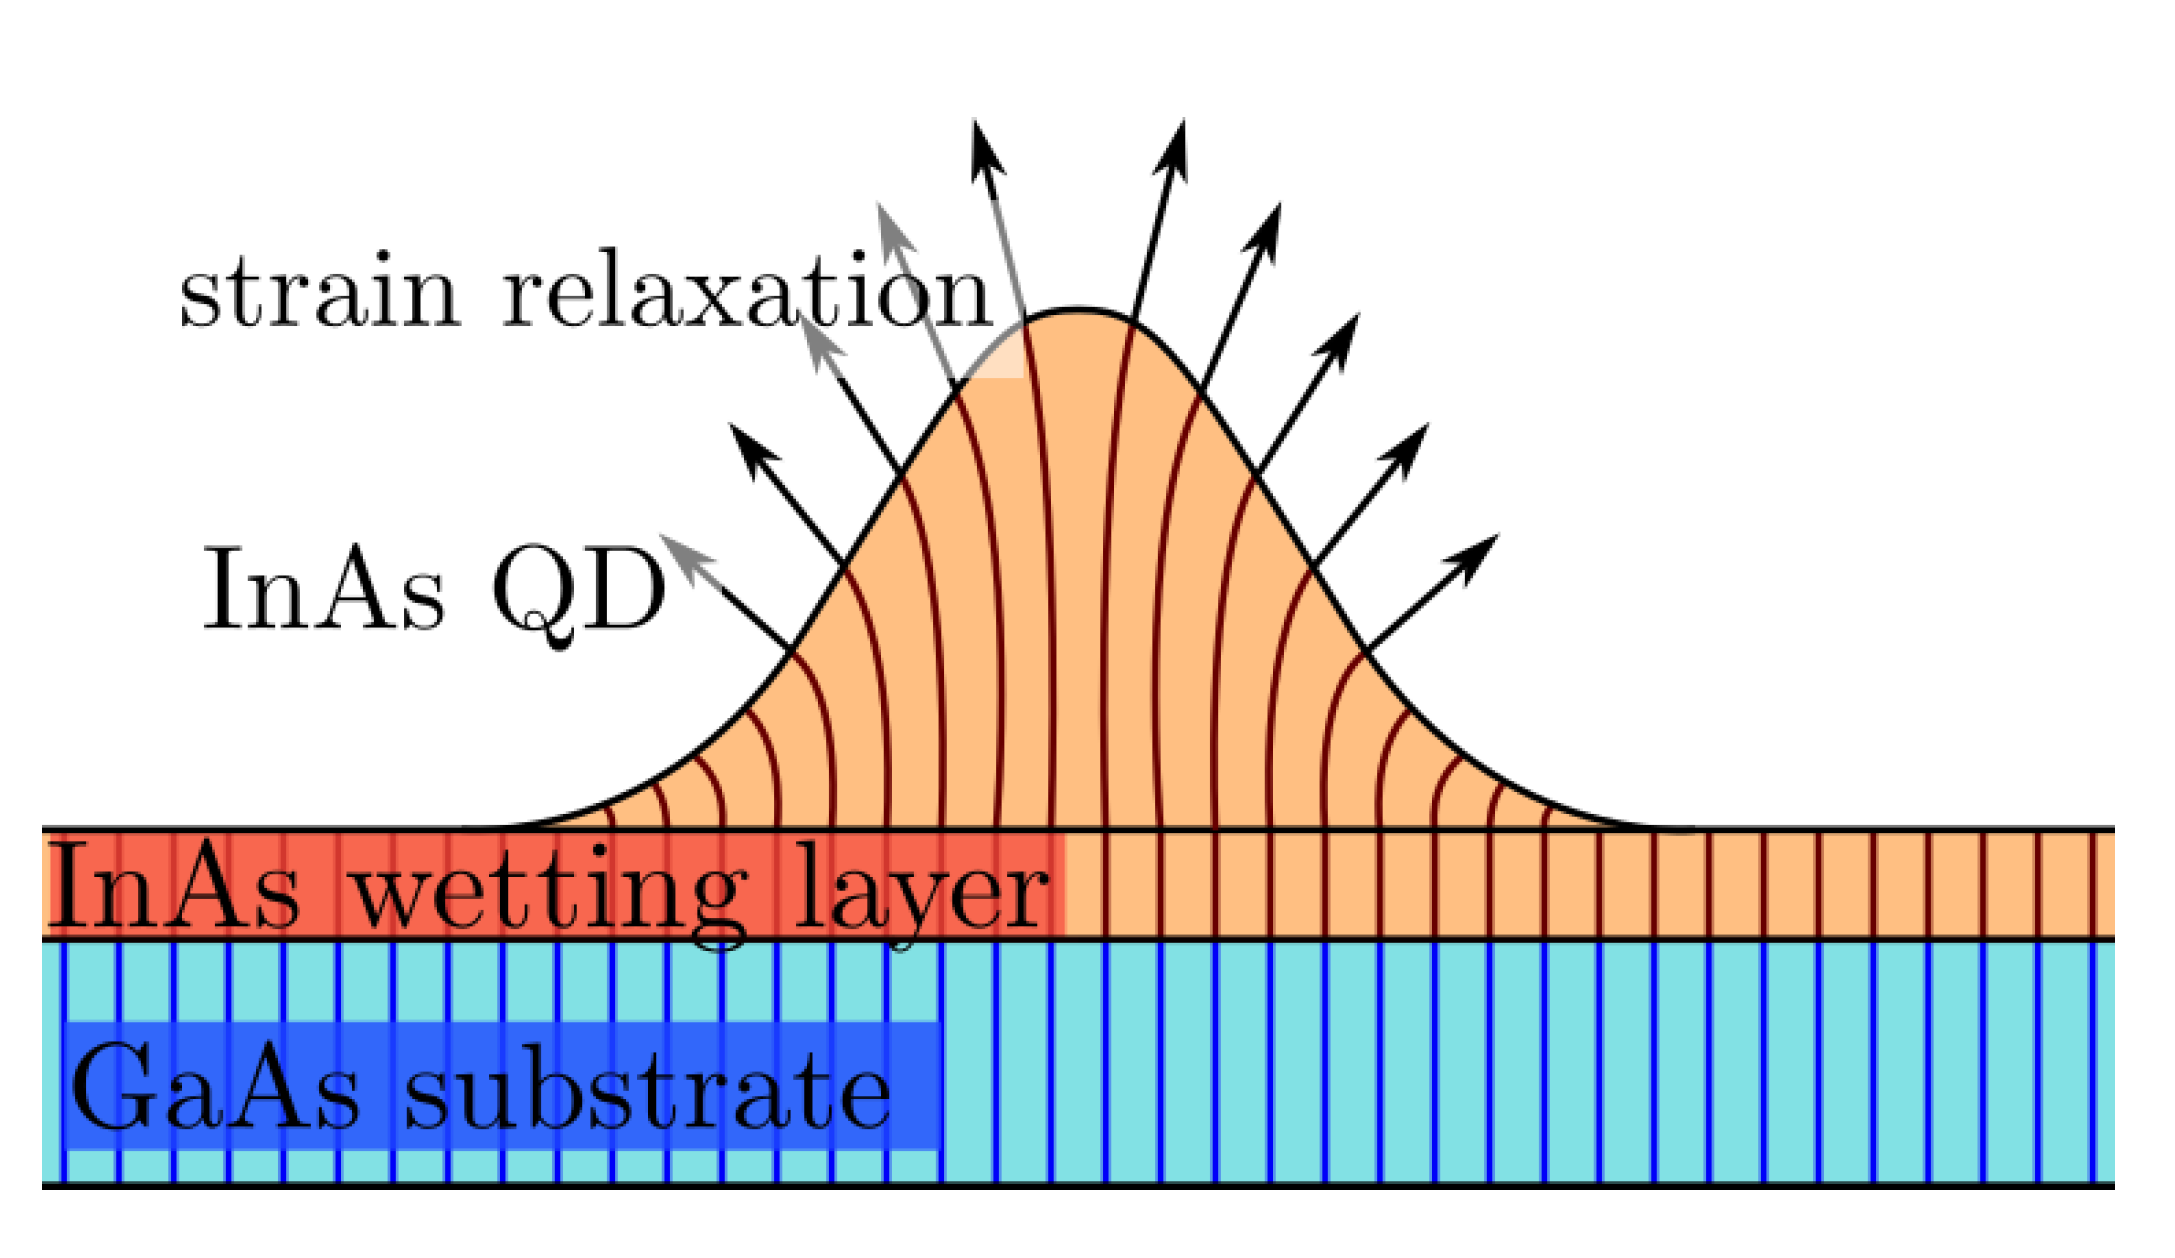
\includegraphics[width = 0.45\textwidth]{Abbildungen/QD_Schema.png}
    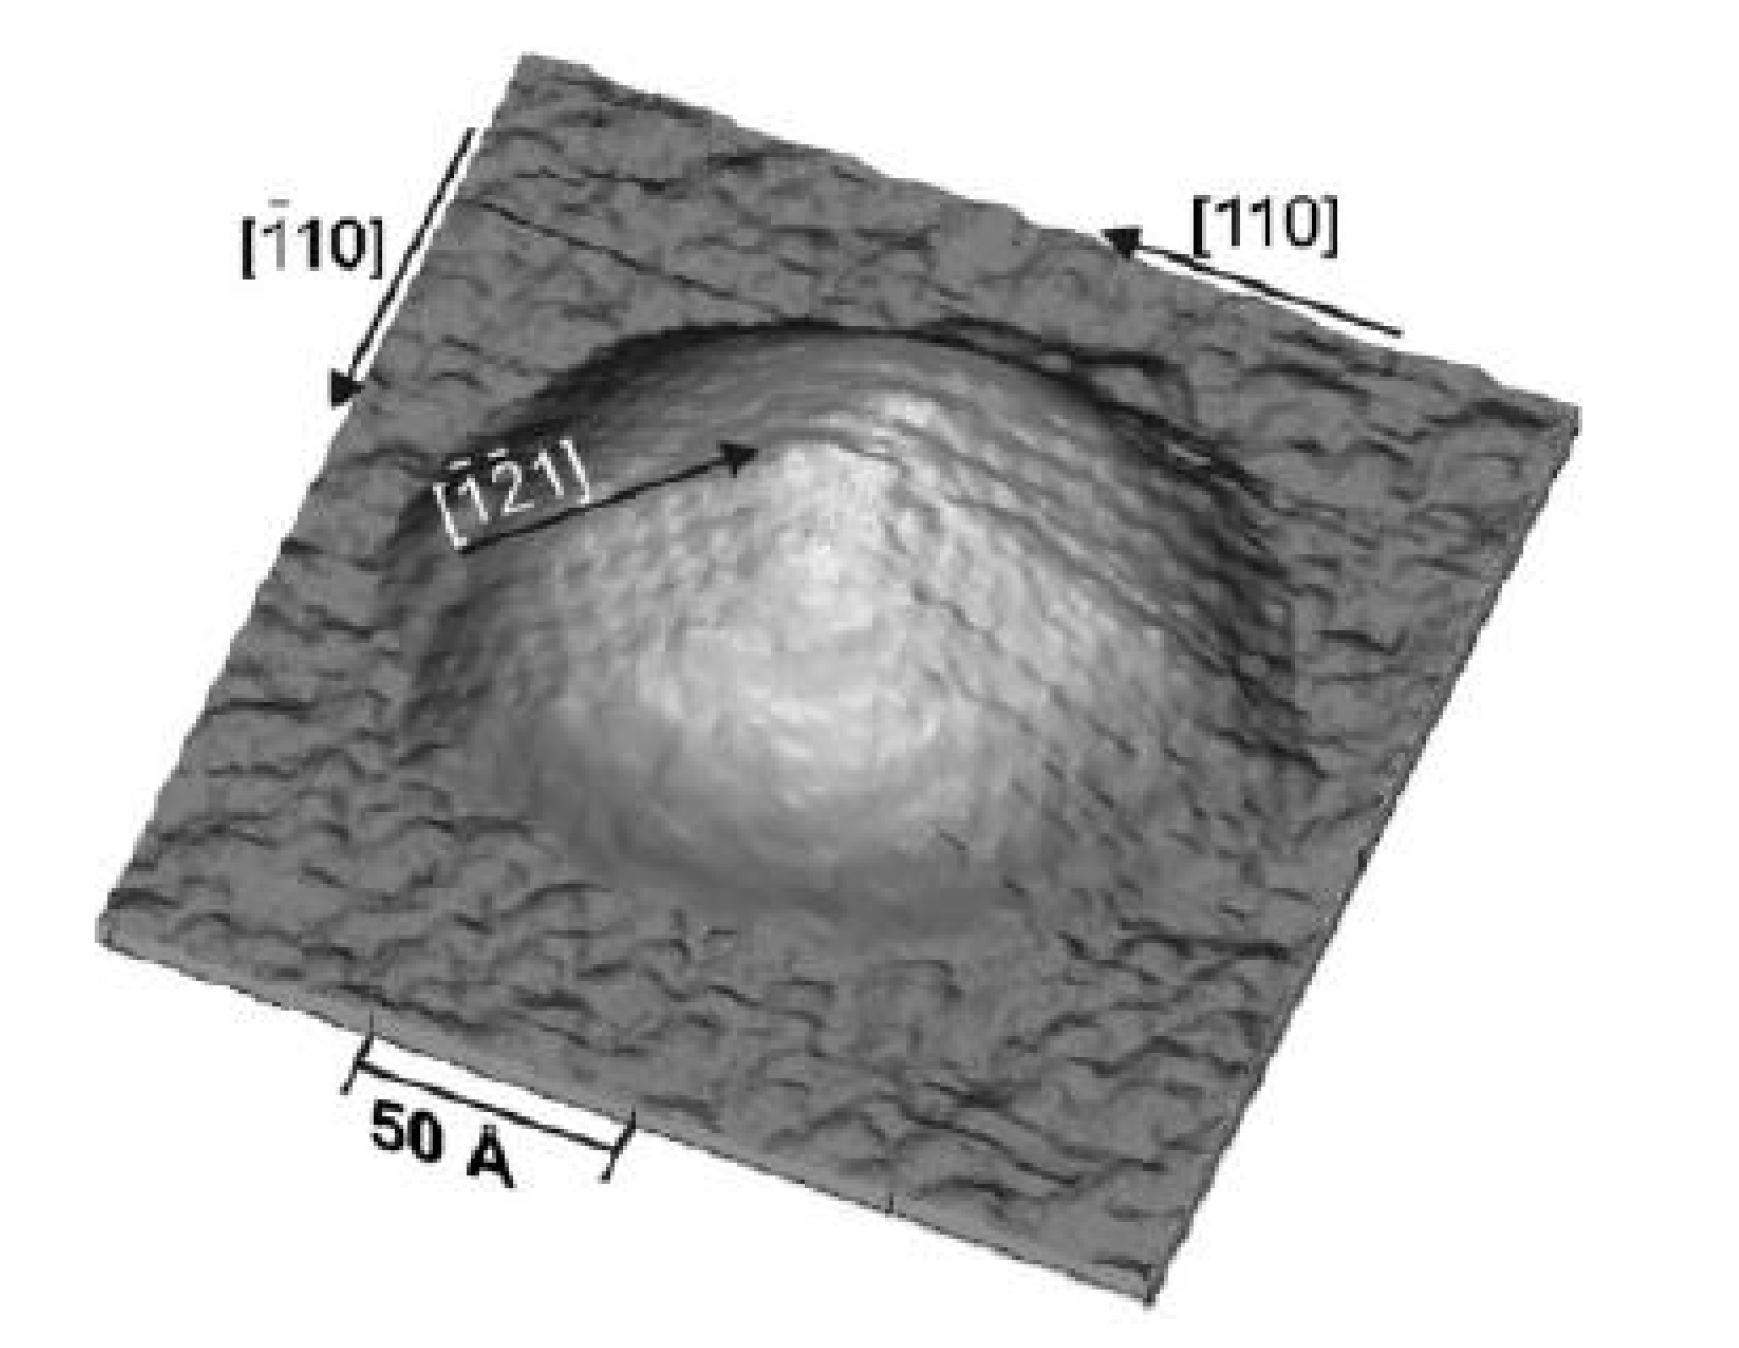
\includegraphics[width = 0.45\textwidth]{Abbildungen/einQD.png}
    \caption{Automatisch aufgelöstes Bild eines InAs-Quantenpunktes}
    \label{fig:QD_Schema}
\end{figure}

\noindent Die hier betrachten Quantenpunkte sind nanoskopische Halbleiterstrukturen, die wie ein dreidimensionaler Potentialtopf fungieren
und einzelne Ladungsträger wie Elektronen oder Löcher einfangen können.\\
Die Stranski-Krastnov-Methode ist eine weitverbreitete Methode um Quantenpunkte zu erzeugen, dabei ist die Idee zwei Materialien mit 
unterschiedlicher Gitterkonstante mittels Molekularstrahlepitaxie aufeinander wachsen zu lassen. Der Kürze Halber lässt es sich 
beispielhaft an den beiden Materialien InAs und GaAs erklären, denn dabei wird eine InAs-Schicht auf ein GaAs-Substrat wachsen gelassen, 
wobei die Gitterkonstante des InAs etwa 7\% größer ist, wodurch Spannung zwischen beiden Materialien entsteht. \\
\noindent Diese Spannung bewirkt eine Formationen von InAs-Inseln wie in \autoref{fig:QD_Schema} zu sehen, die nur wenige zehn 
Nanometer groß sind, und verändert selbst die elektronische Eigenschaften, hauptsächlich den elektrische Feldgradienten des 
Quantenpunktes. Nun wird GaAs auf das ganze Substrat gewachsen, so dass die InAs-Inseln vollständig von 
dem GaAs umschlossen sind. Diese umschlossenen InAs-Inseln bilden dann explizit den Quantenpunkt.\\
\begin{figure}
   \centering
    \includegraphics[width = 0.45\textwidth]{Abbildungen/QD_Energiebänder.png}
    \caption{Schematische räumliche Bandstruktur eines In(Ga)As/GaAs-Quantenpunktes mit den relevanten Bändern und einem 
    gefangenem Ladungsträger}
    \label{fig:QD_Bandstruktur}
\end{figure}

\noindent Das GaAs, welches den In(Ga)As-Quantenpunkt umschließt, fungiert als Potentialtopf, denn die Energiebandlücke des InAs ist 
signifikant kleiner als die des GaAs. Nun kann ein einzelnes Elektron räumlich einfangen werden und durch die Lokalisierung 
die Wechselwirkung mit dem Substrat unterdrückt werden. Dadurch ist nur noch die Hyperfeinstruktur, also die Wechselwirkung mit den 
umliegenden Kernspins die dominante Wechselwirkung, wodurch die Dekohärenzzeit verlängert werden kann. Dies ist vorteilhaft, da 
eine kurze Dekohärenzzeit seit Beginn ein Hauptproblem bei der Realisierung des Quantencomputers ist.\\
In \autoref{fig:QD_Bandstruktur} ist zu erkennen, dass einzelne Elektronen (oder Löcher)
im InAs auf bestimmte Energieniveaus gefangen sind, ähnlich wie in einem Potentialtopf.\\
Quantenpunkte werden deshalb auch als "künstliche Atome" bezeichnet, da ganz in Analogie zu Atomen diskrete Enerigieniveaus 
von den eingefangen Elektronen besetzt werden können.

\chapter{Zentralspinmodell}

\begin{wrapfigure}{r}{0.4\textwidth}
    \centering
    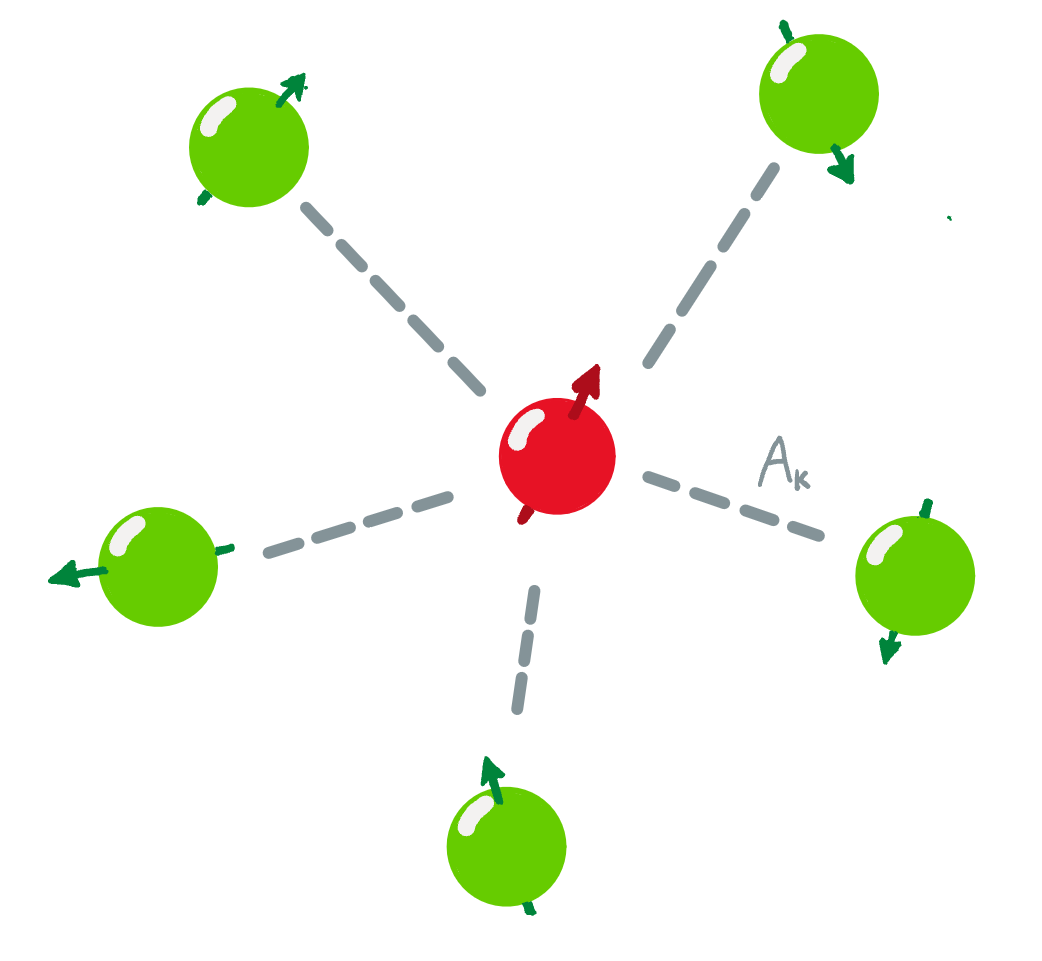
\includegraphics[width = 0.35\textwidth]{Abbildungen/CSM_Schema_Salem.png}
    \caption{Schematischer Aufbau des Zentralspinmodell mit dem Elektronenspins (Rot) und den in direkter Umgebung liegenden 
    Kernspins (Grün) und einer Kopplungskonstante $A_k$}
    \label{fig:CSM}
\end{wrapfigure}
%CSM: https://iopscience.iop.org/article/10.1088/1367-2630/16/6/065023
Im folgenden wird das \textbf{Zentralspinmodell} zur Beschreibung der Spindynamik des Quantenpunktes verwendet. Dabei werden die Interaktionen des 
Elektronenspins mit dem externen Magnetfeld $\vec{B}$ und den umliegenden Kernspins $\hat{\vec{I}}_k$ über eine Heisenbergkopplung $A_k$ berücksichtigt.
Die Kernspins wechselwirken dabei auch mit dem äußeren Magnetfeld, aber die Wechselwirkung untereinander wird vernachlässigt.
\begin{align}
    \overline{\hat{H}}_{CSM} &= \mu_B\thinspace g_e \vec{B}\hat{\vec{S}} +  \sum_{k=1}^{N}\mu_k\thinspace g_k\vec{B}\hat{\vec{I}}_k + \sum_{k=1}^{N} A_k \hat{\vec{S}}\hat{\vec{I}}_k
\end{align}
Dabei entspricht anders als beim freien Elektron der g-Faktor eines Elektron im Quantenpunkt nicht mehr 2, sondern ca. 0,555\cite{PMID:17901328}.
Das Kernmagneton $\mu_k= 5,05 \cdot 10^{27} \frac{J}{T}$ ist etwa 1800 Mal kleiner als das Bohrsche 
Magneton $\mu_B = 9.27 \cdot 10^{24} \frac{J}{T}$\cite{Dyakonov2008-ub}. Die g-Faktoren $g_k$ können für alle Kernspins der 
Einfachheit halber als gleich angenommen werden. \\

\section{charakteristische Zeitskala}
Wenn 



\begin{align}
    T^* &= \frac{1}{\sqrt{\sum_k A_k^2\langle \hat{I}_k^2 \rangle}}
\end{align}
Nun kann der dimensionslose Hamiltonian $\hat{H}_{CSM} = T^*\thinspace\overline{\hat{H}}_{CSM}$ definiert werden:
\begin{align}
    \hat{H}_{CSM} &= \vec{b}\hat{\vec{S}} +  \sum_{k=1}^{N}z_k\vec{b}\hat{\vec{I}}_k + \sum_{k=1}^{N} \alpha_k \hat{\vec{S}}\hat{\vec{I}}_k
\end{align}
% \langle\Psi(t) \mid \dot{\Psi}(t)\rangle
mit $\vec{b}=T^*\mu_B\thinspace g_e \vec{B}$ und $\alpha_k = T^* A_k$. Das Verhältnis zwischen Elektronen-und Kern-Zeemanspaltung ist 
durch $z_k=T^*\frac{\mu_I g_k}{\mu_B g_e}$ definiert.



\chapter{Variationsprinzip}
Es gibt viele Ansätze den Hamiltonian des Zentralspinmodells zu lösen, die von der exakten Lösung über 
semiklassischen Ansätzen\cite{PhysRevB.65.205309,PhysRevB.94.094308,PhysRevB.70.205327,NatalieJaeschke} bishin zum
Chebychev Expansionstheorem reichen\cite{PhysRevB.89.045317}, welche ihre eigenen Vor- und Nachteile beherbergen. 
Gerade bei einer großen Anzahl von Kernspins ist eine exakte quantenmechanische Lösung nicht anwendbar. Deshalb finden semiklassische Ansätze Verwendung, 
die eine Abweichung zur exakten Lösung in Kauf nehmen, um dafür mehr Spins behandeln zu können. In dieser Arbeit wird das Time-Dependent Variatonal 
Principle, kurz TDVP, zur Lösung verwendet. Im folgenden werden komplex konjugierte Variablen $\muk$ mit einem Oberbalken notiert.

\textbf{Historische Randnotiz}\\
Dirac (1930) hat als Erster das Variationsprinzip zur Lösung der zeitabhängigen Schrödingergleichung unter unkommentierten Annahmen vorgestellt; 
diese Annahmen sind in P. A. M. Dirac und P. A. M."Mathematical Proceedings of the Cambridge Philosophical Society 26, 376 (1930)"\cite{Dirac1930-fc,Mott1934-lg} 
zu finden und werden im Rahmen dieser Bachelorarbeit nicht explizit erläutert. \\
Viele Physiker haben versucht Diracs Annahmen zu deuten, darunter P. Kramer, der Diracs Variationsprinzip als ein Wirkungsfunktional 
(siehe Gl. (\ref{Wirkungsfunktional})) interpretiert (TDVP) \cite{noauthor_2008-dn} und dadurch wie unten skizziert die Euler-Lagrange-Gleichungen hergeleitet hat.
Frenkel (1934) hat Diracs Ansatz dementgegen als Minimierungsbedinung (siehe Gl. (\ref{Residuum})) und dadurch Orthogonalprojektion interpretiert ( 
Dirac-Frenkel Variational Principle, kurz DFVP) und 
bezieht sich dabei auf den Appendix der russischen Übersetzung von Diracs Buch als den Ursprung seines Argumentes\cite{Mott1934-lg}.
Diese geometrische Interpretation wurde der Kürze halber vornehmlich unten in der Herleitung verwendet. Beide Interpretationen bzw. Ansätze
sind äquivalent zueinander unter milden Bedingungen\cite{BROECKHOVE1988547}, die für gewöhnlich erfüllt sind.

Eine explizite Herleitung ist in Referenz \cite{noauthor_2008-dn} und \cite{Haegeman_2011} zu finden.
Die zeitabhängige Schrödingergleichung kann durch Extermalisierung des Wirkungsfunktionals
\begin{align}\label{Wirkungsfunktional}
    S\{\overline{\Psi}(t),\Psi(t)\} &=  \int_{t_1}^{t_2}dt \thinspace L(\overline{\Psi}(t),\Psi(t),t)
\end{align}
mit der Lagrange-Funktion und der normierten Wellenfunktion $\ket{\Psi}$:
\begin{align}\label{Lagrange}
    L\left(\overline{\Psi}(t), \Psi(t), t\right)=\frac{i}{2}\langle\Psi(t) \mid \dot{\Psi}(t)\rangle-\frac{i}{2}\langle\dot{\Psi}(t) \mid \Psi(t)\rangle-\langle\Psi(t)|\hat{H}(t)| \Psi(t)\rangle
\end{align}
hergeleitet werden. Der Kürze halber wird die explitzite Zeitabhängigkeit von $\hat{H}$ vernachlässigt und damit auch die von $L$. Stationarität der Wirkung 
$\delta S \overset{!}{=} 0$ unter der unabhängigen Variation von $\ket{\Psi}$ und $\bra{\Psi}$ im vollen Hilbertraum $H$ reproduziert die zeitabhängige 
Schrödingergleichung (und ihr Konjugiertes).\

Die Essenz des Variationsprinzips findet sich bei der Beschränkung auf einen Unterraum bzw. Mannigfaltigkeit $M\subset H$, wobei 
immer noch die Variation von $\ket{\Psi}$ und $\bra{\Psi}$ eine stationäre Lösung liefert, wodurch die Zeitentwicklung des Zustandes $\ket{\Psi} \in M$
definiert ist. Zusätzlich beschränken wir nun die Variation auf die Tangentialebene von $M$ am Zustand $\ket{\Psi}$. Um die Tangentialebene ordentlich 
definieren zu können, kann die Mannigfaltigkeit $M$ parametrisiert werden als   
\begin{align}
    M &= \{\ket{\Psi(\vec{\mu})}|\vec{\mu}\in \mathbb{C}^n\},
\end{align}
wodurch die Zeitabhängigkeit auf die analytischen und komplexen Parameter $\mu_i(t)$ ausgelagert wird; bzw. anti-analytischen Abhängigkeit für 
$\bra{\Psi(\vec{\muk})}$. Somit kann die Tangentialebene am Zustand $\ket{\Psi}$ definiert werden als  
\begin{align}
    T_{\mu(t)}M &= span\{\ket{\partial_{\mu_i}\Psi}, i = 1,...,n\}.
\end{align}
Anmerkung: Es wird die Konvention $\bra{\partial_{\overline{\mu_j}}\Psi} = \left(\thinspace\ket{\partial_{\mu_j}\Psi}\thinspace\right)^\dagger$ verwendet.

Nun kann durch die direkte Variation der Parameter $\vec{\muk}(t)\rightarrow \vec{\muk}(t) + \delta\vec{\muk}$ und der Stationaritätsbedingung 
$\delta S = 0$ die Euler-Lagrange-Gleichungen hergeleitet werden. Äquivalent zur Variation können die Parameter $\mu_i$ geometrisch hergeleitet
werden, indem das Residuum der Schrödingergleichung bzw. der Abstand zwischen der Schrödingergleichung und der Tangentialebene $T_{\mu(t)}M$ 
\begin{align}\label{Residuum}
    || i\underbrace{\sum_k \dot{\mu}_k\ket{\partial_{\mu_k}\Psi}}_{\frac{d}{dt}\ket{\Psi}} - \hat{H}\ket{\Psi} || 
\end{align}
minimiert wird. Dies gelingt durch eine Orthogonalprojektion von $\hat{H}\ket{\Psi}$ auf die Tangentialebene $T_{\mu(t)}M$. Dafür definieren wir den 
Projektionsoperator
\begin{align}
    \hat{P}_{T_{\mu}M} &= \sum_{i,j}\ket{\partial_{\mu_i}\Psi}(G_{i,j})^{-1}\bra{\partial_{\muk_j}\Psi}
\end{align}
Dabei taucht hier die inverse Grammatrix 
\begin{align}
    G_{ij} &= \bra{\partial_{\overline{\mu_i}}\Psi}\ket{\partial_{\mu_j}\Psi}. 
\end{align}
auf, damit u.a. die Projektionsoperatoreigenschaft $\hat{P}_{T_{\mu}M}^2=\hat{P}_{T_{\mu}M}$ 
erfüllt ist. Über einen Koeffizientenvergleich zwischen
\begin{align}
    \hat{P}_{T_{\mu}M}\hat{H}\ket{\Psi} = \sum_{i,j}\left((G_{i,j})^{-1}\ 
    \langle\partial_{\muk_j}\Psi|\hat{H}\ket{\Psi}\right)\ket{\partial_{\mu_i}\Psi}
\end{align} 
und aus (\ref{Residuum})
\begin{align}
    i\sum_k \dot{\mu}_k\ket{\partial_{\mu_k}\Psi}
\end{align}
zu den Zustandsvektoren $\ket{\partial_{\mu_i}\Psi}$ ergeben sich schlussendlich die \textbf{Euler-Lagrange-Gleichungen} für den normierten Fall:
\begin{align}
    i\dot{\mu_i} &= \sum_{j}\left(G_{ij}\right)^{-1}\thinspace \langle\partial_{\muk_j}\Psi|\hat{H}\ket{\Psi}
\end{align}
Da in dieser Arbeit ein nicht-normierter Wellenfunktionsansatz verwendet wird, ist der verallgemeinerte Fall von besonderem Interesse. Die Zeitentwicklung
des Hamiltonian ist unitär und somit normerhaltend, was aber nicht mehr für die Projektion gilt. Wir
können die modifizierte Lagrange-Funktion $\widetilde{L}(\overline{\Psi}(t), \Psi(t)) = \frac{L(\overline{\Psi}(t), \Psi(t))}{\langle \Psi(t)|\Psi\rangle}$
definieren und unter Berücksichtigung der Parametrisierung erhalten wir
\begin{align}
        \widetilde{L}(\vec{\muk}(t),\vec{\mu}(t)) &= \frac{i}{2}\sum_j\left(\dot{\mu_j}(t)\partial_{\mu_j} + \dot{\muk_j}(t)\partial_{\muk_j}\right)
        ln(\langle\Psi(\vec{\muk}(t))|\Psi(\vec{\mu}(t))\rangle) - \mathcal{H}(\vec{\muk}(t),\vec{\mu}(t))
\end{align}
mit der effektiven Hamilton-Funktion
\begin{align}
    \mathcal{H} = \frac{\bra{\Psi}\hat{H}\ket{\Psi}}{\N}.
\end{align}
Stationarität unter Variation $\vec{\muk}(t)\rightarrow \vec{\muk}(t) + \delta\vec{\muk}$ ergeben die 
verallgemeinerten Euler-Lagrange-Gleichungen. Hier kann aber wieder eine geometrische Interpretation zur Herleitung verwendet werden. Unter einer 
infinitisimalen Verrückung in $\ket{\Psi}$-Richtung des Zustandes $\ket{\Psi}$ ändern sich Phase und Norm, um Normerhaltung zu bewahren, wird von jedem 
Tangentenvektor $\ket{\partial_{\mu_i}\Psi}$ die Komponente entlang $\ket{\Psi(\vec{\mu})}$ subtrahiert. Dieses Abziehen kann durch den 
Projektionsoperator 
\begin{align}
    \hat{P}_0 &= \hat{1} - \frac{\ket{\Psi(\vec{\mu})}\bra{\Psi(\vec{\mu})}}{\langle\Psi(\vec{\muk}(t))|\Psi(\vec{\mu}(t))\rangle}
\end{align}
realisiert werden, wenn alle Tangentenvektoren $\ket{\partial_{\mu_i}\Psi}$ mit $\hat{P}_0\ket{\partial_{\mu_i}\Psi}$ ausgetauscht werden.
Dadurch ergibt sich unter Berücksichtigung der Normierung die \textbf{modifizierte Gram-Matrix}
\begin{align}
    \tilde{G}_{ij} &= \frac{\langle\partial_{\muk_i}\Psi|\hat{P}_0\ket{\partial_{\mu_j}\Psi}}{\N}  \nonumber \\
    &= \frac{\langle\partial_{\overline{\mu_i}}\Psi|\partial_{\mu_j}\Psi\rangle}{\N}
    - \frac{\langle\partial_{\muk_i}\Psi|\Psi\rangle\langle\Psi|\partial_{\mu_j}\Psi\rangle}{\N^2}
\end{align}
und aus $ \langle\partial_{\muk_j}\Psi|\hat{H}\ket{\Psi}$ unter Berücksichtigung der Normierung ergibt sich ebenfalls
\begin{align}
    \frac{\langle\partial_{\muk_j}\Psi|\hat{P}_0\thinspace\hat{H}\ket{\Psi}}{\langle\Psi|\Psi\rangle}    
                &= \frac{\langle\partial_{\mu_j}\Psi|\hat{H}\ket{\Psi}}{\N} 
                - \frac{\langle\partial_{\mu_j}\Psi|\Psi\rangle\langle\Psi|\hat{H}\ket{\Psi}}{\N^2} \nonumber \\
                &= \partial_{\muk_j}\mathcal{H}                
\end{align}

Und damit erhalten wir wie beim direkten Ausrechnen der stationären Variation des Wirkungsfunkionals mit der modifizierten 
Lagrangefunktion $\widetilde{L}$, die \textbf{verallgemeinerten Euler-Lagrange-Gleichungen}:
\begin{align}\label{verallgemeinerter_Euler_Lagrange}
    i\dot{\mu}_i &= \sum_{j}\left(\tilde{G}_{ij}\right)^{-1}\thinspace \partial_{\overline{\mu}_j}\mathcal{{H}}
\end{align}
%%%%%%%%%%%%%%%%%%%%%%%%%%%%%%%%
%%%%%%%%%%%%%%%%%%%%%%%%%%%%%%%%  Ansatz_Wellen-Funktiom
%%%%%%%%%%%%%%%%%%%%%%%%%%%%%%%%
\newpage
\section{Wahl der Wellenfunktion für einen semiklassischen Ansatz}
\begin{wrapfigure}{r}{0.3\textwidth}
    \centering
    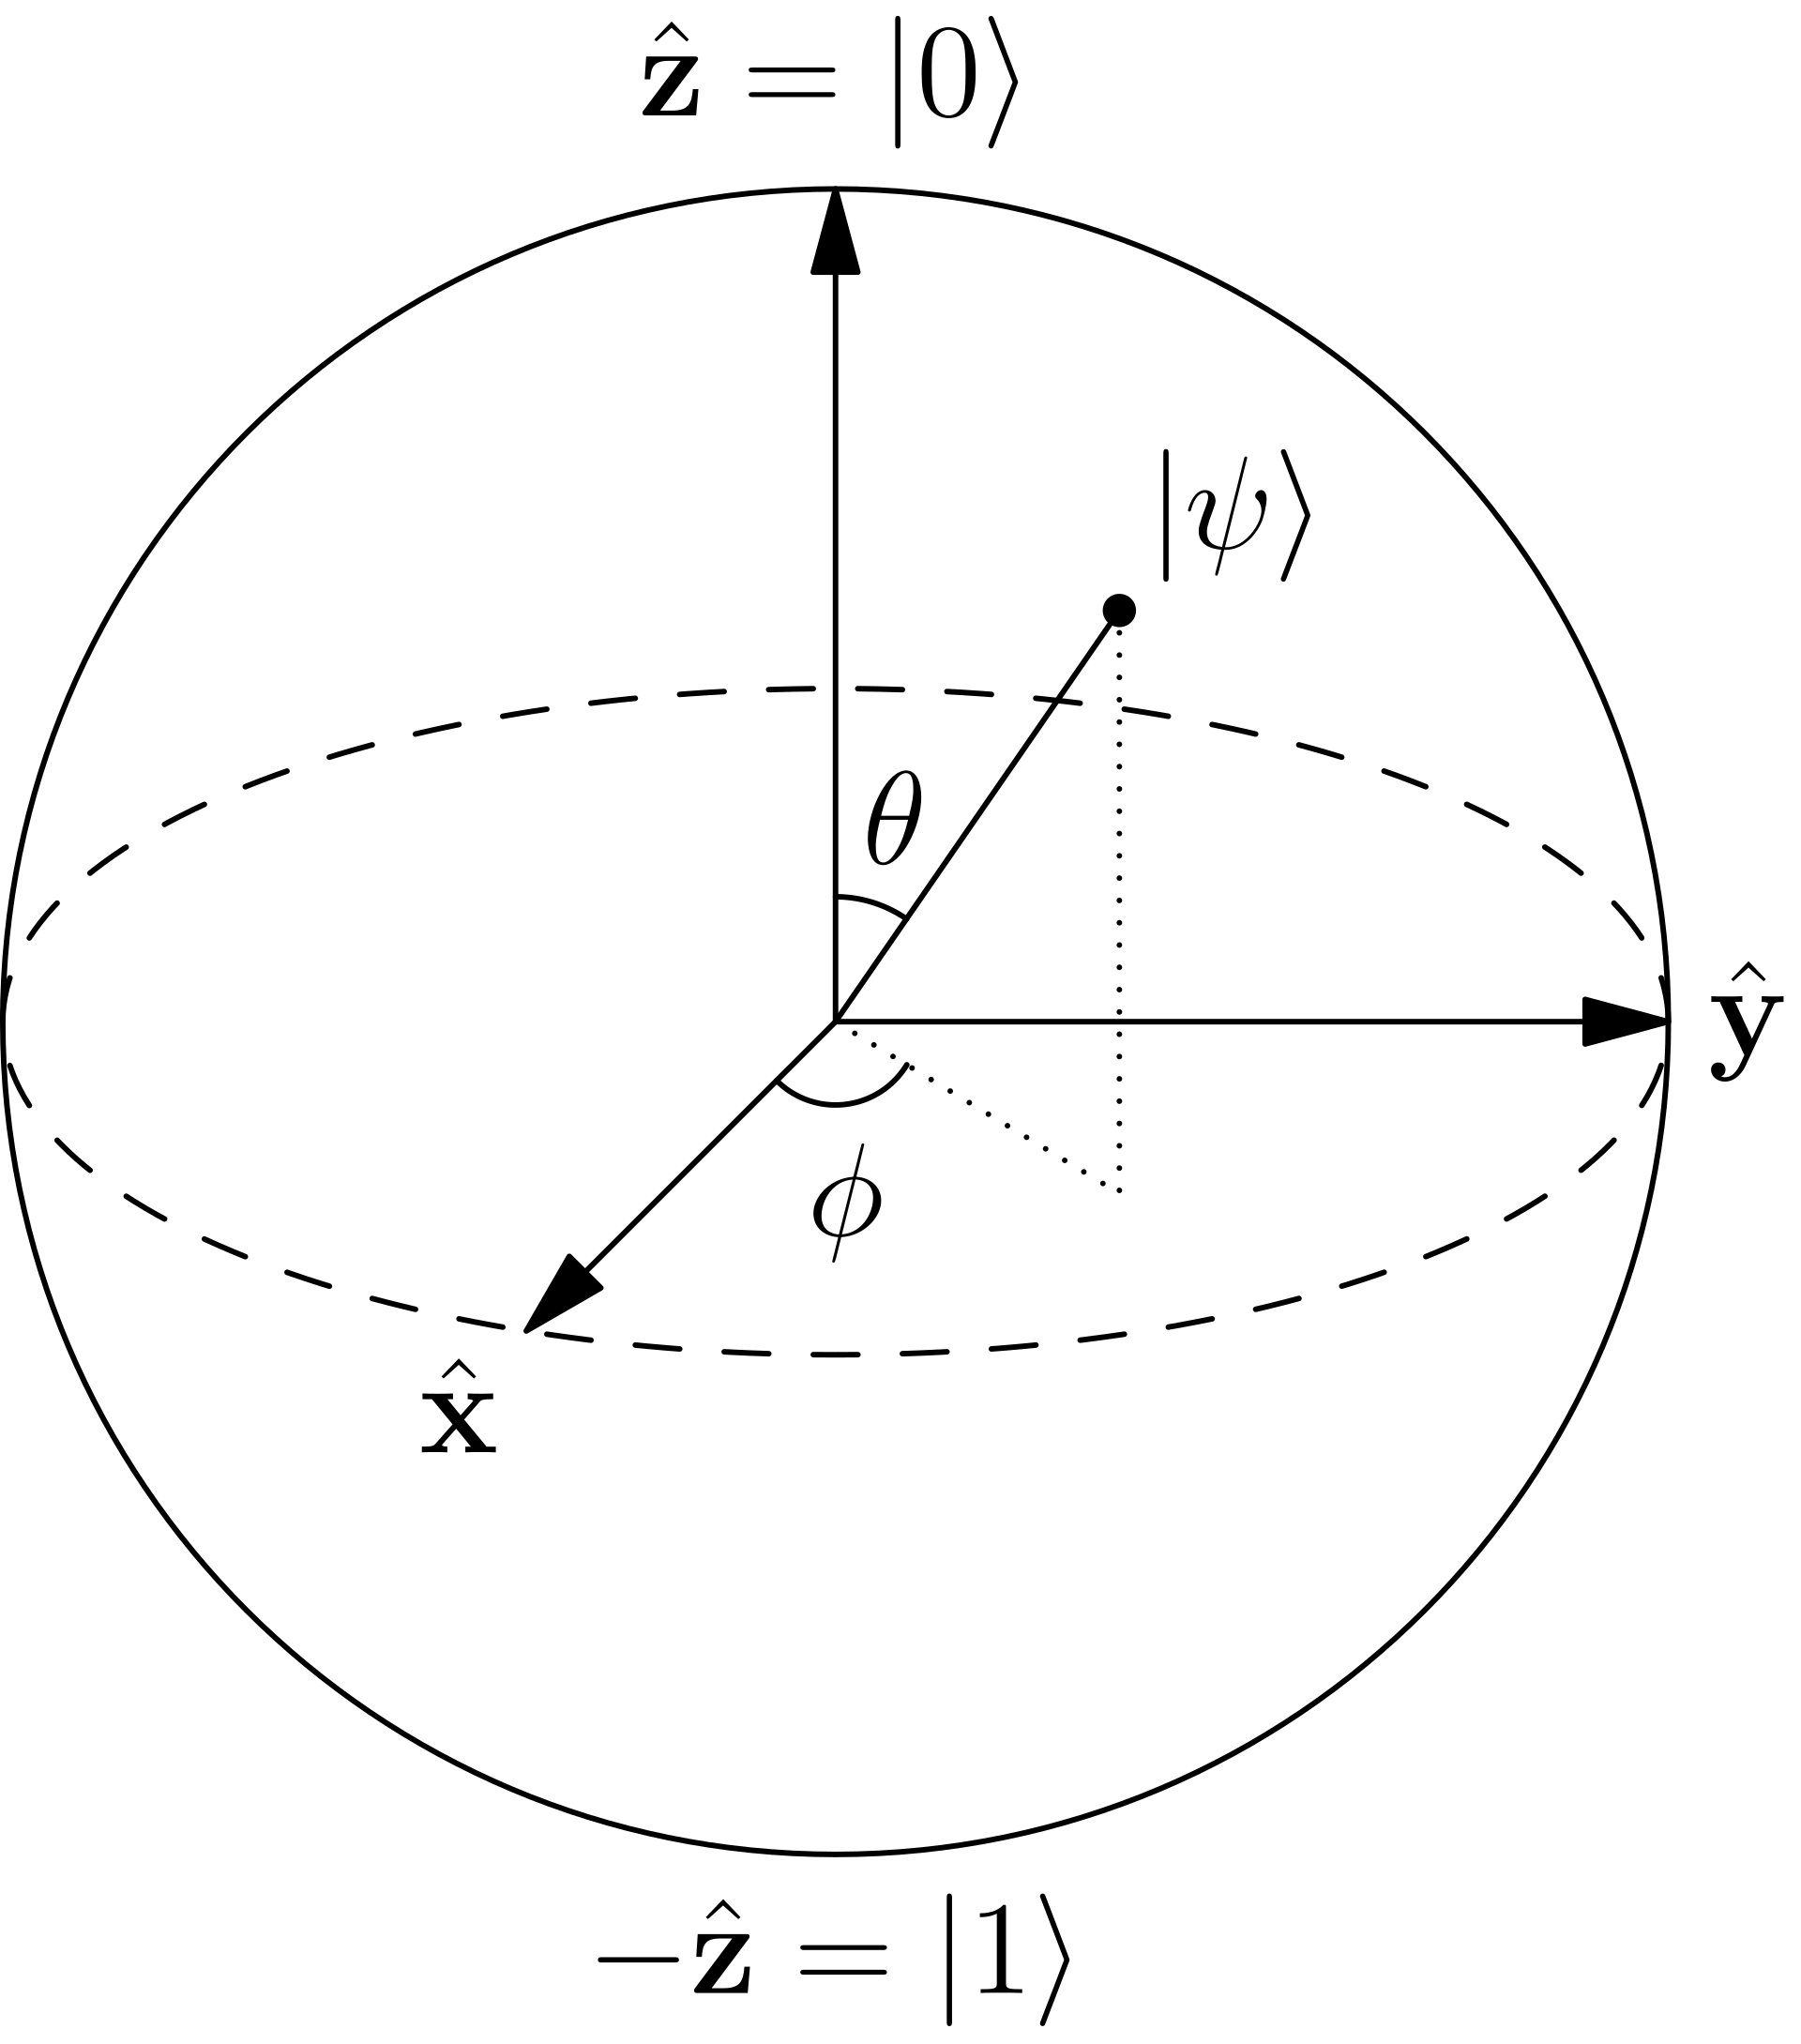
\includegraphics[width = 0.3\textwidth]{Abbildungen/Bloch_sphere_wikimedia.png}
    \caption{Schematischer Aufbau einer Bloch-Sphäre. Dabei entspricht $|0\rangle$  gerade $|\uparrow\rangle$ und $|1\rangle$ gerade 
    $|\downarrow\rangle$ \cite{pict}.}
    \label{fig:qubit}
\end{wrapfigure}
Zur Vereinfachung werden alle Kernspins (wie der Elektronenspin) als 1/2-Spins angenommen. 
Wir nutzen die Geometrie des 1/2-Spins aus und verwenden zur Darstellung die bekannte \textbf{Bloch-Sphäre}. 
Ähnlich wie die komplexe e-Funktion dank trigonometrischer Eigenschaften einen Kreis auf der Zahlenebene abbilden kann, ist es auch möglich,
jeden Punkt auf einer Kugeloberfläche zu beschreiben. Die folgende Wellenfunktion 
\begin{align}\label{klassischer_Ansatz}
    \ket{\Psi(\mu_1(t),...,\mu_n(t))} &= \frac{1}{N}\prod_{i=1}^{n} e^{\mu_i\thinspace S_i^-}\ket{\uparrow,...,\uparrow}
\end{align}
mit dem Normierungsfaktor
\begin{align}
    N &= \prod_{i=1}^{n} \frac{1}{\sqrt{1+\mu_i\muk_i}}.
\end{align}
beschreibt gerade einen Produktzustand aus $n$ Bloch-Sphären und wird mit den komplexen Parametern $\mu_i(t)$ parametrisiert. Dabei beschreibt der
Betrag $|\mu|$ die Anteile von $|\uparrow\rangle$ und $|\downarrow\rangle$ in der Wellenfunktion jeweils. Der Zustand $|\uparrow\rangle$ kann durch $\mu=0$ 
und der Zustand $|\downarrow\rangle$ als Grenzwert für $|\mu|\rightarrow \infty$ erreicht werden; dadurch steht der Betrag $|\mu|$ in Beziehung mit
mit dem Winkel $\Theta$ in \autoref{fig:qubit} über $\theta = 2\tan^{-1}(|\mu|)$. Das komplexe Argument von $\mu$ beschreibt dabei die Phase der 
Zustände und steht deshalb ebenfalls in Beziehung mit dem Winkel $\phi$ in \autoref{fig:qubit}.\\
Dieser Ansatz ist die Basis für weitere Korrekturen, die im späteren Verlauf verwendet werden können, um quantenmechanische Effekte berücksichtigen zu 
können.\\
Es wird der Ansatz aus Gl. (\ref{klassischer_Ansatz}) ohne den Normierungsfaktor verwendet, da das TDVP nur eine analytische Wellenfunktion variieren kann,
der Normierungsfaktor ist aber durch das Auftauchen von $\mu_i$ und dem konjugierten $\muk_i$ nicht analytisch. Es kann aber immer noch auf die 
verallgemeinerte Euler-Lagrange-Gleichungen Gl. (\ref{verallgemeinerter_Euler_Lagrange}) zurückgegriffen werden.\\
%%%%%%%%%
%%%%%%%%%
\section{ein 1/2-Spin im konstanten Magnetfeld}
Zum besseren Verständnis des TDVPs ist die beispielhafte Betrachtung des vereinfachten Falles sehr aufschlussreich. 
Zudem lassen sich Identitäten herleiten, die in die Erweiterung zum \textbf{Zentralspinmodell} Wiederverwendung finden werden. Hierfür wird nur der erste 
Summand des Zentralspinmodells betrachtet:
\begin{align*}
    \ket{\Psi} &= e^{\mu\thinspace S^-}\ket{\uparrow} \\
            &= (1 + \frac{\mu\thinspace S^{-}}{1!} + \frac{\left(\mu\thinspace S^{-}\right)^2}{2!} + ...)\ket{\uparrow}    \\
            &= \ket{\uparrow} + \mu\ket{\downarrow}
\end{align*}
\noindent Im folgenden haben wir uns die Eigenschaft des 1/2-Spins $\left(S^{-}\right)^{n}\ket{\uparrow}=0$  (n = 2,3,...) verwendet.
Dieser Ansatz deckt unter Berücksichtigung der Normierung und der Phasenfreiheit den gesamten Hilbertraum des 1/2-Spins ab
\begin{align}
    \ket{\mu} &= e^{i\phi}\frac{1}{\sqrt{1 + \mu\muk}}\ket{\uparrow} + e^{i\phi}\frac{\mu}{\sqrt{1 + \mu\muk}}\ket{\downarrow}.
\end{align}
Der Hamilton-Operator für einen Spin in einem Magnetfeld $\vec{B}$ lautet
\begin{align}
    \hat{H}_1 &= \vec{b}\hat{\vec{S}} = \left(b_x\hat{S}_x+b_y\hat{S}_y+b_z\hat{S}_z \right) \\
    &= \frac{b_x}{2}\Bigl(\ket{\downarrow}\!\bra{\uparrow}+\ket{\uparrow}\!\bra{\downarrow}\Bigr) \\
    & + \frac{ib_y}{2}\Bigl(\ket{\downarrow}\!\bra{\uparrow}-\ket{\uparrow}\!\bra{\downarrow}\Bigr) \\
    & + \frac{b_z}{2}\Bigl(\ket{\uparrow}\!\bra{\uparrow}-\ket{\downarrow}\!\bra{\downarrow}\Bigr), 
\end{align}
\noindent wobei der Lande-Faktor des freien Elektrones $g_e\approx 2$ ist. 
Der Spin-Vektororperator hat die Form $\hat{\vec{S}}= \frac{1}{2}\left(\hat{\sigma}_x,\hat{\sigma}_y,\hat{\sigma}_z\right)^T$ mit den Pauli-Matrizen 
$\hat{\sigma}_i$.\\ 
und somit ergibt sich der effektive Hamilton-Funktion und seine partielle Ableitung nach $\muk$:
\begin{align}
    \mathcal{H} &= \frac{1}{2}\frac{b_x(\mu +\muk) + ib_y(\muk - \mu) + b_z(1-\mu\muk) }{1+\mu\muk}    \\
    \partial_{\muk} \mathcal{H} &= \frac{1}{2} \frac{b_x(1-\mu^2) + ib_y(1+\mu^2) - 2\mu b_z}{(1+\mu\muk)^2} 
\end{align}
\noindent Im nächsten Schritt wird die von dem Hamiltionian unabhängigen modifizierte Gram-Matrix $G_{ii}$ bestimmt, 
welche in diesem Fall eindimesnional ist.
Damit erhalten wir
\begin{align}
    G_{11} = \frac{1}{\left(1 + \mu\overline{\mu}\right)^2} \text{\space\space bzw.\space\space } G_{11}^{-1} = \left(1 + \mu\overline{\mu}\right)^2
\end{align}
\noindent Einsetzen in die verallgemeinerte Euler-Lagrange-Gleichung \autoref{verallgemeinerter_Euler_Lagrange} liefert:
\begin{align}
    i\dot{\mu_i} &= \sum_{j}\left(G_{ij}\right)^{-1}\thinspace \partial_{\overline{\mu_j}}\mathcal{H} = \left(G_{11}\right)^{-1}\partial_{\muk} \mathcal{H} \\
    &= \frac{b_x}{2}(1-\mu^2) + \frac{i b_y }{2}(1+\mu^2) -\mu b_z   \label{Larmor} \\ 
    \leftrightarrow \dot{\mu} &= \frac{1}{2}(b_y + ib_x)\mu^2 + \frac{1}{2}(b_y - ib_x) +i\mu b_z .
\end{align}
Die normierten \textbf{Spin-Erwartungswerte} $\frac{\bra{\Psi}\hat{\vec{S}}\ket{\Psi}}{\N}$ lauten:
\begin{align}
    \frac{\bra{\Psi}\hat{S_x}\ket{\Psi}}{\N} &= \frac{1}{2}\frac{\muk + \mu}{1+\mu\muk} = \frac{Re[\mu]}{1 + \mu\muk} \\
    \frac{\bra{\Psi}\hat{S_y}\ket{\Psi}}{\N} &= \frac{i}{2}\frac{\muk - \mu}{1+\mu\muk} = \frac{Im[\mu]}{1 + \mu\muk} \\
    \frac{\bra{\Psi}\hat{S_z}\ket{\Psi}}{\N} &= \frac{1}{2}\frac{1 - \mu\muk}{1 + \mu\muk}  .
\end{align}
Unter Verwendung der Identität 
\begin{align}
    \frac{d}{dt}\left(\frac{\bra{\Psi}\hat{S_\alpha}\ket{\Psi}}{\N}\right) &= \partial_{\mu}\left[\frac{\bra{\Psi}\hat{S_\alpha}\ket{\Psi}}{\N}\right]\dot{\mu} 
    + \partial_{\muk}\left[\frac{\bra{\Psi}\hat{S_\alpha}\ket{\Psi}}{\N}\right]\dot{\muk}\label{dS_dt}
\end{align}
ergeben sich die Bewegungsgleichungen der Form
\begin{align}
    \frac{d}{dt}\left(\frac{\bra{\Psi}\hat{\vec{S}}\ket{\Psi}}{\N}\right) &= \vec{b} \cross \left(\frac{\bra{\Psi}\hat{\vec{S}}\ket{\Psi}}{\N}\right).
\end{align}
Dies entspricht wie zu erwarten der \textit{Larmor-Präzession}.

%%%%%%%%%%%%%%%%%%%%%%%%%%%%%%%%%%%%












\section{Zwei Spins: Klassischer Ansatz}
Der vollständige zwei 1/2-Spin-Hilbertraum wird aufgespannt durch
\begin{align}
    \ket{\Psi} &= \alpha_1\ket{\uparrow\uparrow} + \alpha_2 \ket{\downarrow\uparrow} + \alpha_3\ket{\downarrow\uparrow} + \alpha_4\ket{\downarrow\downarrow}
\end{align}
mit den unabhängigen, komplexen Parametern $\alpha_i$.
\noindent Mit dem klassischen Ansatz $\ket{\Psi} = \ket{\Psi(\mu_1, \mu_2)}$ aus Gl. (\ref{klassischer_Ansatz}) ergibt sich: 
\begin{align}
    \ket{\Psi} &= e^{\mu_1 \hat{S}^{-}}e^{\mu_2 \hat{I}^{-}}\ket{\uparrow,\uparrow} \nonumber\\
                &= \ket{\uparrow \uparrow} +\mu_1\ket{\downarrow \uparrow} + \mu_2\ket{\uparrow \downarrow} + \mu_1\mu_2\ket{\downarrow\downarrow}\nonumber\\
                &= \underbrace{\left(\ket{\uparrow}_1 + \mu_1\ket{\downarrow}_1\right)}_{\ket{\Psi_1}}\underbrace{\left(\ket{\uparrow}_2 + \mu_2\ket{\downarrow}_2\right)}_{\ket{\Psi_2}}  .
\end{align}
Dabei wurde $\hat{S}_1^{-} = \hat{S}^{-}$ und $\hat{S}_2^{-} = \hat{I}^{-}$ gesetzt, um die Unterscheidung zwischen Elektronen- und Kernspin hervorzuheben.
Wird die Phasenfreiheit und die Normierung berücksichtigt und unter einem komplexen Parameter $\mu_0$ zusammengefasst
\begin{align}\label{ueberlapp_klassisch}
    \underbrace{Ne^{i\phi}}_{=\mu_0}\ket{\Psi} &= \underbrace{\mu_0}_{\alpha_1}\ket{\uparrow \uparrow} 
    + \underbrace{\mu_0\mu_1}_{\alpha_2}\ket{\downarrow \uparrow} + \underbrace{\mu_0\mu_2}_{\alpha_3}\ket{\uparrow \downarrow} 
    + \underbrace{\mu_0\mu_1\mu_2}_{\alpha_4}\ket{\downarrow\downarrow},
\end{align}
lässt sich erkennen, dass $\alpha_1$,$\alpha_2$ und $\alpha_3$ unabhängig sind, aber $\alpha_4$ gerade 
von $\alpha_1$,$\alpha_2$ und $\alpha_3$ abhängig ist. Dadurch wird der Hilbertraum auf einen Unterraum beschränkt. Der Hamiltonoperator 
des Zentralspinmodells für den zwei 1/2-Spin Fall lautet
\begin{align}\label{zweiSpinHamilton}
    \hat{H}_{CSM} &= \vec{b}\hat{\vec{S}} +  z\vec{b}\hat{\vec{I}} + \alpha \hat{\vec{S}}\hat{\vec{I}}\space.
\end{align}
Damit ergibt sich für die effektive Hamilton-Funktion: 
\begin{align}
    \mathcal{H} &= \frac{\bra{\Psi}\hat{H}_1\ket{\Psi}+ \bra{\Psi}\hat{H}_2\ket{\Psi} +\bra{\Psi}\hat{H}_3\ket{\Psi}}{\N}
\end{align}
mit
\begin{align}
   \bra{\Psi}\hat{H_1}\ket{\Psi} &= \frac{1}{2}(1+\mu_2\muk_2)\left(b_x(1-\mu_1^2) + ib_y(1+\mu_1^2) - 2\mu_1 b_z\right)\\
   \bra{\Psi}\hat{H_2}\ket{\Psi} &= \frac{z}{2}(1+\mu_1\muk_1)\left(b_x(1-\mu_2^2) + ib_y(1+\mu_2^2) - 2\mu_2 b_z\right)\\
   \bra{\Psi}\hat{H}_3\ket{\Psi} &= \frac{\alpha}{4}\left[( \mu_1 + \muk_1)( \mu_2 + \muk_2) - (\mu_1-\muk_1)(\mu_2 - \muk_2) + (1-\mu_1\muk_1)(1-\mu_2\muk_2)\right]
\end{align}  
Und wir erhalten die partiellen Ableitungen:
\begin{align}
    \partial_{\muk_1}\mathcal{H} &= \underbrace{\frac{1}{2(1+\mu_1\muk_1)^2}[b_x(1-\mu_1^2) + ib_y(1+\mu_1^2) - b_z\mu_1]}_{= \partial_{\muk_1} \frac{\bra{\Psi}\hat{H}_1 + \hat{H}_2\ket{\Psi}}{\N}} \nonumber\\
    &+ \underbrace{\frac{\alpha}{2}\frac{(\mu_2 -\mu_1)(1+\mu_1\muk_2)}{(1+\mu_1\muk_1)^2(1+\mu_2\muk_2)}}_{= \partial_{\muk_1} \frac{\bra{\Psi}\hat{H}_3\ket{\Psi}}{\N}}\\
    \partial_{\muk_2}\mathcal{H} &= \underbrace{\frac{z}{2(1+\mu_2\muk_2)^2}[b_x(1-\mu_2^2) + iB_y(1+\mu_2^2) - B_z\mu_2]}_{= \partial_{\muk_2} \frac{\bra{\Psi}\hat{H}_1 + \hat{H}_2\ket{\Psi}}{\N}} \nonumber \\
    &+ \underbrace{\frac{\alpha}{2}\frac{(\mu_1 -\mu_2)(1+\mu_2\muk_1)}{(1+\mu_1\muk_1)(1+\mu_2\muk_2)^2}}_{= \partial_{\muk_2} \frac{\bra{\Psi}\hat{H}_3\ket{\Psi}}{\N}}\space .
\end{align}
Zudem ergibt sich die modifizierte Gram-Matrix
\begin{align}
    G &=
    \begin{pmatrix}
        (1+\mu_1\muk_1)^2 & 0 \\
        0 &(1+\mu_2\muk_2)^2
    \end{pmatrix} \\
    G^{-1} &=
    \begin{pmatrix}
        \frac{1}{(1+\mu_1\muk_1)^2} & 0 \\
        0 &\frac{1}{(1+\mu_2\muk_2)^2}
    \end{pmatrix}\space ,
\end{align}
die diesmal zweidimensional ist.
\noindent Nun können die Euler-Lagrange-Gleichungen aufgestellt werden:
\begin{align}
    i\dot{\mu}_1 &= \sum_{j}\left(G_{1j}\right)^{-1}\thinspace \partial_{\overline{\mu_j}}\mathcal{H}  \\
    &=\underbrace{\frac{1}{2}b_x(1-\mu_1^2) + \frac{i}{2}b_y(1+\mu_1^2) -\mu_1 b_z}_{\text{Ein-Spin-Präzession um } \vec{b}} +\underbrace{\frac{\alpha}{2} \frac{(\mu_2-\mu_1)(1+\mu_1\muk_2)}{1+\mu_2\muk_2}}_{\text{Ein-Spin-Präzession um } \frac{\bra{\Psi}\hat{\vec{I}}\ket{\Psi}}{\N}  } \label{DGL_klassisch_S}   
\end{align}
und in analoger Weise 
\begin{align}
    i\dot{\mu}_2 &= \underbrace{\frac{z}{2}b_x(1-\mu_2^2) + \frac{iz}{2}b_y(1+\mu_2^2) -\mu_2 z b_z}_{\text{Ein-Spin-Präzession um } \vec{b}} +\underbrace{\frac{\alpha}{2} \frac{(\mu_1-\mu_2)(1+\mu_2\muk_1)}{1+\mu_1\muk_1}}_{\text{Ein-Spin-Präzession um } \frac{\bra{\Psi}\hat{\vec{S}}\ket{\Psi}}{\N}  }.\label{DGL_klassisch_I}
\end{align}
\noindent Aufgrund der Linearität der Differentialgleichungen ist beim Vergleich mit Gl. (\ref{Larmor}) zu erkennen, dass es sich bei den ersten
beiden Summanden um die Lösung aus dem Ein-Spin-Fall im Magnetfeld handelt. Nun fehlt es noch zu beweisen, dass der letztere Summand tatsächlich die 
Präzession um den Spin-Erwartungswert des jeweilig anderen Spins beschreibt bzw. das Overhausener Feld. Dies kann gezeigt werden, wenn in 
der Gl. (\ref{Larmor}) die $b_{x,y,z}$ durch $\alpha\frac{\bra{\Psi}\hat{I}_{x,y,z}\ket{\Psi}}{\N}$ ausgetauscht
werden
\begin{align}
     \frac{\alpha}{2}\left[\underbrace{\frac{1}{2}\frac{\mu_2 + \muk_2}{1+\mu_2\muk_2}}_{\frac{\bra{\Psi}\hat{I}_x\ket{\Psi}}{\N}}(1-\mu_1^2) 
     + i \underbrace{\frac{i}{2}\frac{\muk_2 -\mu_2}{1+\mu_2\muk_2}}_{\frac{\bra{\Psi}\hat{I}_y\ket{\Psi}}{\N}}(1+\mu_1^2) 
     - 2\mu_1\underbrace{\frac{1}{2}\frac{1-\mu_2\muk_2}{1+\mu_2\muk_2}}_{\frac{\bra{\Psi}\hat{I}_z\ket{\Psi}}{\N}} \right],
\end{align}
denn einfaches Auflösen führt ebenfalls zu
\begin{align}
    \frac{\alpha}{2} \frac{(\mu_2-\mu_1)(1+\mu_1\muk_2)}{1+\mu_2\muk_2}.
\end{align}
Dies entspricht gerade dem letzten Summanden in Gl. (\ref{DGL_klassisch_S}) und (\ref{DGL_klassisch_I}).
Hier lässt sich erkennen, dass die $\alpha\frac{\bra{\Psi}\hat{I_i}\ket{\Psi}}{\N}$ die Rolle des Magnetfeldes $\vec{b}$ in der Ein-Spin-Lösung 
übernehmen. Wir erhalten dann aus Symmetriegründen:
\begin{align}
    \frac{d}{dt}\left[\frac{\bra{\Psi}\hat{\vec{S}}\ket{\Psi}}{\N}\right] &= \left(\vec{b} + \alpha \frac{\bra{\Psi}\hat{\vec{I}}\ket{\Psi}}{\N}\right)\cross\frac{\bra{\Psi}\hat{\vec{S}}\ket{\Psi}}{\N} \label{DGL_1}\\
    \frac{d}{dt}\left[\frac{\bra{\Psi}\hat{\vec{I}}\ket{\Psi}}{\N}\right] &= \left(z\vec{b} + \alpha \frac{\bra{\Psi}\hat{\vec{S}}\ket{\Psi}}{\N}\right)\cross\frac{\bra{\Psi}\hat{\vec{I}}\ket{\Psi}}{\N} \label{DGL_2}
\end{align}


%%%%%%%%%%%%% Quantenkorrektur




\section{Modifizierter Ansatz: Quantenkorrektur}
\noindent Wie im vorherigen Abschnitt zu sehen, erhalten wir eine klassiche Lösung. Um eine genauere Lösung zu erhalten, 
führen wir einen weiteren Korrekurparameter $\mu_{12}$ ein, wodurch ein größerer Unterraum des zwei 1/2-Spin-Hilbertraumes aufgespannt 
wird, mit der Hoffnung im Gegensatz zum klassischen Ansatz die Verschränkung zu berücksichtigen:
\begin{align}
    \ket{\Psi(\mu_1,\mu_2,\mu_{12})} &= e^{\mu_1 S_1^-}e^{\mu_2 S_2^-}e^{\mu_{12} S_1^-S_2^-}\ket{\uparrow,\uparrow}\\
                                    &= \ket{\uparrow \uparrow} +\mu_1\ket{\downarrow \uparrow} + \mu_2\ket{\uparrow \downarrow} + (\mu_1\mu_2 + \mu_{12})\ket{\downarrow \downarrow}
\end{align}
Wird  die Phasenfreiheit und die Normierung berücksichtigt und unter einem komplexen Parameter $\mu_0$ zusammengefasst
\begin{align}
    \underbrace{Ne^{i\phi}}_{=\mu_0}\ket{\Psi} &= \underbrace{\mu_0}_{\alpha_1}\ket{\uparrow \uparrow} 
    + \underbrace{\mu_0\mu_1}_{\alpha_2}\ket{\downarrow \uparrow} + \underbrace{\mu_0\mu_2}_{\alpha_3}\ket{\uparrow \downarrow} 
    + \underbrace{\mu_0(\mu_1\mu_2 + \mu_{12})}_{\alpha_4}\ket{\downarrow\downarrow}
\end{align}
Im Gegensatz zum klassischen Ansatz lässt sich erkennen, dass alle Parameter $\alpha_i$, einschließlich $\alpha_4$, unabhängig sind. Somit ist der gesamte
Hilbertraumabgedeckt und die exakte Lösung zu erwarten.\\
Aufgrund der Tatsache, dass bei einem $\vec{b}$-Feld in beliebiger Richtung, sich die Rechnung und Ergebnisse außerordentlich verkomplizieren, ohne 
wirklich neue Erkenntnis zu bringen, wird das Magnetfeld in z-Richtung ausgerichtet. Somit vereinfacht sich der 
Hamiltonian (\ref{zweiSpinHamilton}) zu:
\begin{align}\label{Hamiltonian_Bz}
    \hat{H} &= \vec{b}\hat{\vec{S}}_z +  z\vec{b}\hat{\vec{I}}_z + \alpha \hat{\vec{S}}\hat{\vec{I}}
\end{align}
Mit diesem Ansatz erhalten wir nach längerer Rechnung den modifizierten Hamiltonian:
\begin{align}
    \mathcal{H} &= \frac{\bra{\Psi}\hat{H}_1\ket{\Psi} +\bra{\Psi}\hat{H}_2\ket{\Psi} + \bra{\Psi}\hat{H}_3\ket{\Psi}}{\N}
\end{align}
mit 
\begin{align}
    \bra{\Psi}\hat{H}_1\ket{\Psi} &=  \frac{b}{2}\left[ 1- \mu_1\muk_1 + \mu_2\muk_2 - (\mu_1 \mu_2 + \mu_{12})(\overline{\mu_1\mu_2} + \muk_{12})\right]\\
    %
    \bra{\Psi}\hat{H}_2\ket{\Psi} &=  \frac{z b}{2}\left[ 1- \mu_2\muk_2 + \mu_1\muk_1 - (\mu_1 \mu_2 + \mu_{12})(\overline{\mu_1\mu_2} + \muk_{12})\right] \\
    %
    \bra{\Psi}\hat{H}_3\ket{\Psi} &= \frac{\alpha}{4}[2(\muk_1\mu_2 + \mu_1\muk_2) + 1 - \mu_1\muk_1 - \mu_2\muk_2 + (\mu_1 \mu_2 + \mu_{12})(\overline{\mu_1\mu_2} + \muk_{12})].
\end{align}
\noindent Damit folgen für die partiellen Ableitungen nach den konjugierten Parameter
\begin{align}
    \partial_{\muk_1} \mathcal{H} &= 
    -b \frac{\mu_1(1+\mu_2\muk_2)^2 + \muk_2\mu_{12}}{\N^2}\nonumber\\
    &+z b \frac{\muk_{12}(\mu_1\mu_2 + \mu_{12})}{\N^2}\nonumber\\
    &+\frac{\alpha}{2}\frac{(\mu_2-\mu_1)(\mu_1\muk_2+1)(1+\mu_2\muk_2)+\muk_{12}(\mu_1\mu_2 + \mu_{12}) + \mu_{12}\muk_2}{\N^2}\label{dH_Q1} \\
    %
    \partial_{\muk_2} \mathcal{H} &= 
    +b \frac{\muk_{12}(\mu_1\mu_2 + \mu_{12})}{\N^2} \nonumber\\
    &-z b \frac{\mu_2(1+\mu_1\muk_1)^2 + \muk_1\mu_{12}}{\N^2} \nonumber\\
    &+\frac{\alpha}{2}\frac{(\mu_1-\mu_2)(\mu_2\muk_1+1)(1+\mu_1\muk_1)+\muk_{12}(\mu_1\mu_2 + \mu_{12}) + \mu_{12}\muk_1}{\N^2} \\
    %
    \partial_{\muk_{12}} \mathcal{H} &= 
    -b\frac{(\mu_1\mu_2+\mu_{12})(1+\mu_2\muk_2)}{\N^2} \nonumber\\
    &-zb\frac{(\mu_1\mu_2+\mu_{12})(1+\mu_1\muk_1)}{\N^2} \nonumber\\
    &+\frac{\alpha}{2}\frac{(\muk_1-\muk_2)(\mu_1-\mu_2)(\mu_1\mu_2+\mu_{12})}{\N^2}\label{dH_Q12}
\end{align}
\noindent und für die Gram-Matrix erhalten wir:
\begin{align}\label{Gram_Korrektur}
    G &=
    \begin{pmatrix}
        (1+\mu_1\muk_1)^2 + \mu_{12}\muk_{12} & -\mu_1^2\muk_{12} - \muk_2^2\mu_{12} &  \mu_2(1+\mu_2\muk_2)-\muk_1\mu_{12}\\
        -\mu_2^2\muk_{12} - \muk_1^2\mu_{12} &(1+\mu_2\muk_2)^2 + \mu_{12}\muk_{12} & \mu_1(1+\mu_1\muk_1)-\muk_2\mu_{12}\\
        \muk_2(1+\mu_2\muk_2)-\mu_1\muk_{12} & \muk_1(1+\mu_1\muk_1)-\mu_2\muk_{12} & 1 + \mu_1\muk_1 + \mu_2\muk_2
    \end{pmatrix}\frac{1}{\N^2} .
\end{align}
Somit lassen sich die Bewegungsgleichungen der Parameter explizit aufschreiben:
\begin{align}
    i\dot{\mu}_1 &= G_{1,1}^{-1}\thinspace \partial_{\muk_1}\mathcal{H} + G_{1,2}^{-1}\thinspace\partial_{\muk_2}\mathcal{H} + G_{1,3}^{-1}\thinspace\partial_{\muk_3}\mathcal{H}\label{QK_DGL1} \\
    i\dot{\mu}_2 &= G_{2,1}^{-1}\thinspace\partial_{\muk_1}\mathcal{H} + G_{3,2}^{-1\thinspace}\partial_{\muk_2}\mathcal{H} + G_{2,3}^{-1}\thinspace\partial_{\muk_3}\mathcal{H} \\
    i\dot{\mu}_{12} &= G_{3,1}^{-1}\thinspace\partial_{\muk_1}\mathcal{H} + G_{3,2}^{-1}\thinspace\partial_{\muk_2}\mathcal{H} + G_{3,3}^{-1}\thinspace\partial_{\muk_3}\mathcal{H} \label{QK_DGL3}.
\end{align}
Die Ergebnisse sind deutlich komplexer als für den klassischen Ansatz. Zur Herleitung der Spindynamik würden sich deshalb numerische Methoden zur Lösung der 
Differetialgleichung ergeben, wobei die modifizierte Gram-Matrix Gl. (\ref{Gram_Korrektur}) der Kürze halber auch numerisch invertiert werden kann, da eine 
direkte Inversion einen noch kompliziertere Matrix ergeben würde mit wenig neuer Erkenntnis.

\chapter{Diskussion}
Hier wird nun die klassische Lösung für den Zwei-Spin-Fall mit der exakten quantenmechanischen Lösung verglichen.
\section{Quantenmechanische Lösung}
Für die exakte quantenmechanische Lösung des Hamiltonoperators Gl. (\ref{Hamiltonian_Bz}) wird der Hamiltonian diagonalisiert über die Basis:
\begin{align}
    \ket{1} &= \ket{\uparrow\uparrow}   \\
    \ket{2} &= \ket{\downarrow\downarrow} \\
    \ket{3} &= \frac{1}{\sqrt{2}N_1}\left[(\epsilon_1+1)\ket{\uparrow\downarrow} +(\epsilon_1-1)\ket{\downarrow\uparrow} \right]\\
    \ket{4} &= \frac{1}{\sqrt{2}N_2}\left[(\epsilon_2+1)\ket{\uparrow\downarrow} +(\epsilon_2-1)\ket{\downarrow\uparrow} \right]
\end{align}
mit $\epsilon_{1,2} = \frac{\alpha \pm \sqrt{b^2(1-z)^2+\alpha^2} }{b(z-1)} $ und $N_{i} = \sqrt{\epsilon_i^2 + 1}$. Die dazugehörigen Eigenenergien lauten:
\begin{align}
    E_1 &= \frac{b(1+z)}{2} + \frac{\alpha}{4}\\
    E_2 &= -\frac{b(1+z)}{2} + \frac{\alpha}{4}\\
    E_3 &= -\frac{\alpha}{4} + \frac{\sqrt{\alpha^2 + b^2(1-z)^2}}{2}\\
    E_4 &= -\frac{\alpha}{4} - \frac{\sqrt{\alpha^2 + b^2(1-z)^2}}{2}.
\end{align}
\noindent Über den Zeitentwicklungsoperator und einem beliebigen Startzustand $\ket{\Psi_0}$, lässt sich die zeitabhängige Wellenfunktion 
$|\Psi(t)\rangle = e^{-i\hat{H}t}|\Psi_0\rangle = \sum_j e^{-i E_j t}|j\rangle\langle j|\Psi_0\rangle$ definieren. Somit ist die Spindynamik
beschrieben über
\begin{align}
    \bra{\Psi}\hat{S}_\alpha\ket{\Psi}(t) &= \sum_{i,j}e^{i(E_i-E_j)t}\bra{i}\hat{S}_\alpha\ket{j}\bra{j}\ket{\Psi_0}\bra{\Psi_0}\ket{i}.
\end{align}
\section{Exemplarischer Vergleich}
\begin{wrapfigure}{r}{0.4\textwidth}
    \centering
    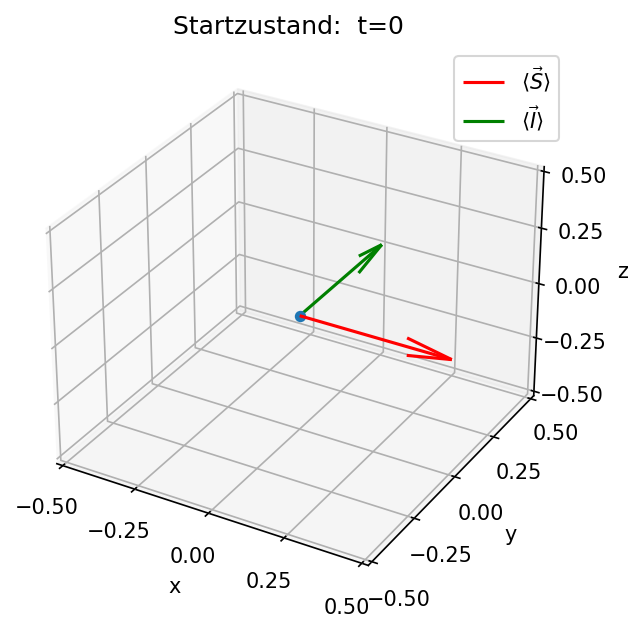
\includegraphics[width = 0.4\textwidth]{Abbildungen/Plot_Vektor_Start.png}
    \caption{gewählter Startzustand in einem 3D-Plot mit rotem Elektronenspinerwartungswert und grünem Kernspinerwartungswert als Vektoren dargestellt}
    \label{fig:Plots_Start}
\end{wrapfigure}
Es wird der Produkt-Startzustand 
\begin{align}
    \ket{\Psi_0}=\frac{1}{2}(\ket{\uparrow}_S + \ket{\downarrow}_S)(\ket{\uparrow}_I + i\ket{\downarrow}_I)
\end{align}
verwendet, welcher Äquivalent zu einem Elektronenspinerwartungswert $\langle\vec{S}\rangle$ entlang der X-Achse und orthogonal
dazu einem Kernspinerwartungswert $\langle\vec{I}\rangle$ entlang der Y-Achse ist, beide auf der X-Y-Ebene liegend wie in \autoref{fig:Plots_Start} zu sehen.
Dieser Startzustand wurde unter all den möglichen Startzuständen gewählt, da dieser einen sehr einfachen und anschaulichen Fall darstellt, denn das Magnetfeld und beide Spinvektoren 
bilden ein Dreibein und gleich zu Beginn ist die Wirkung der Kopplungen untereinander durch die Orthogonalität am stärksten.

Dabei wird zur Lösung der Differentialgleichungen Gl. (\ref{DGL_1}) und Gl. (\ref{DGL_2}) das Runge-Kutta-Verfahren verwendet, da die 
Bewegungsgleichungen die Form besitzen:
\begin{align}
    \frac{d}{dt}\vec{f} &= \vec{f}(\vec{t}) .
\end{align}
%The parameters are chosen to approximately reflect the experimental
%setup given by Greilich et al. [33] and stay the same for the following sections unless
%stated otherwise. In previous comparisons between theory and experiment [49] T
%∗ has
%been found to be T
%∗ ≈ 1 ns
%Die Parameter werden nah am experimentellen Aufbau gegeben von Greilich et al.\cite{PMID:17901328} gewählt, d.h. wir nehmen an,
In vorherigen Vergleichen zwischen Experiment und Theorie ergab sich für die charakteristische Zeit $T^*\approx 1 \thinspace$ns\cite{PhysRevB.89.045317}, 
woraus über Gl. (\ref{charakteristische_Zeit}) für die Heisenbergkopplungskonstante $A = \sqrt{\frac{4}{3}}\cdot 10^9 \frac{1}{s}$ folgt. Des weiteren wird
$z=\frac{1}{800}$ und ein Magnetfeld mit $B = 0.5$ T gewählt. Darüber hinaus wird die Zeitspanne so lang gewählt, dass die Umhüllende der 
summierten Spinlänge $|\langle \left( \vec{S}+\vec{I} \right)\rangle |$  der exakten Lösung in \autoref{fig:Plots_Spinlength} Panel (b) ihr erstes Minimum 
überschreitet.
\begin{figure}[h]
    \centering
    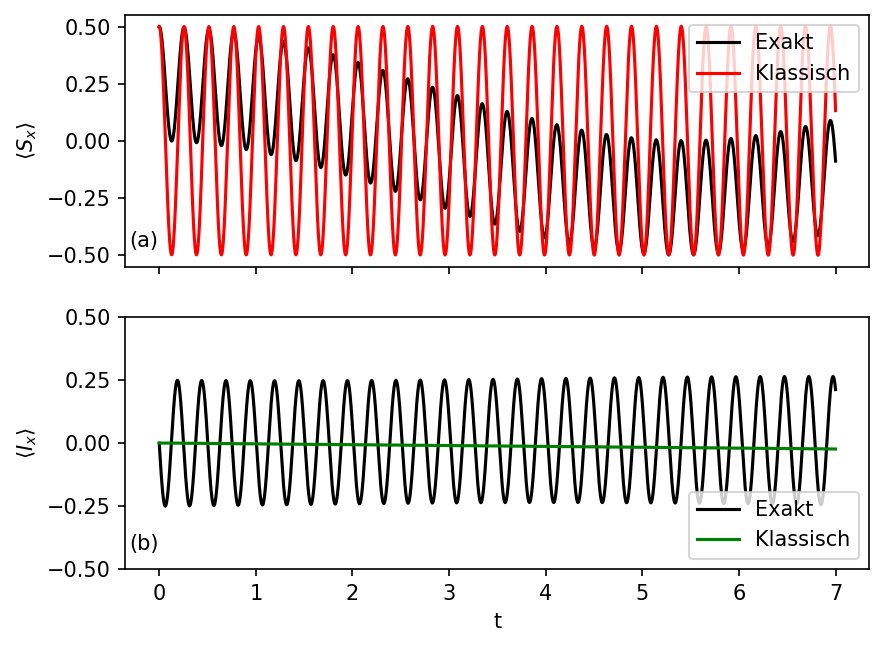
\includegraphics[width = 0.45\textwidth]{Abbildungen/Plot_Sx_index.png}
    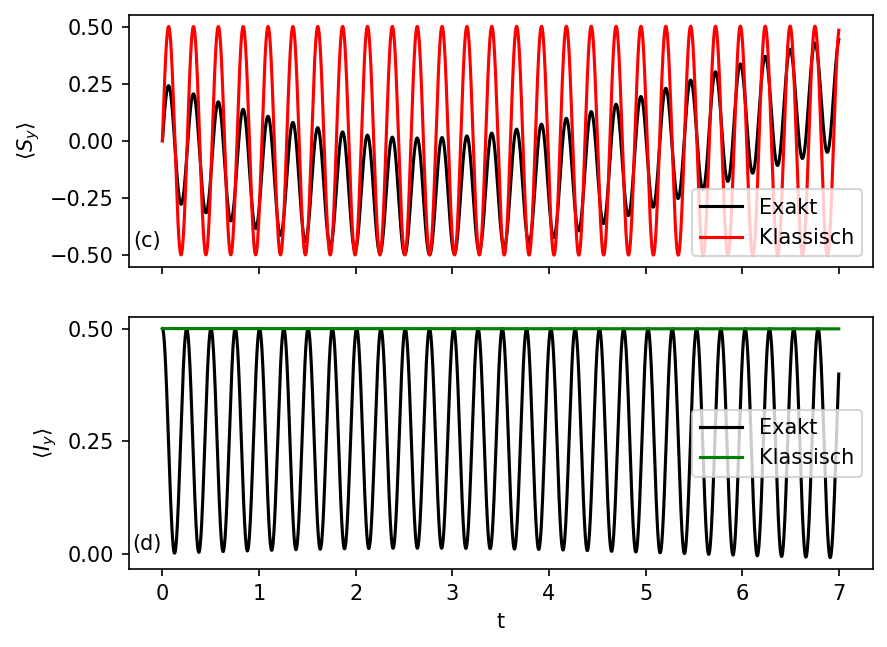
\includegraphics[width = 0.45\textwidth]{Abbildungen/Plot_Sy_index.png}
    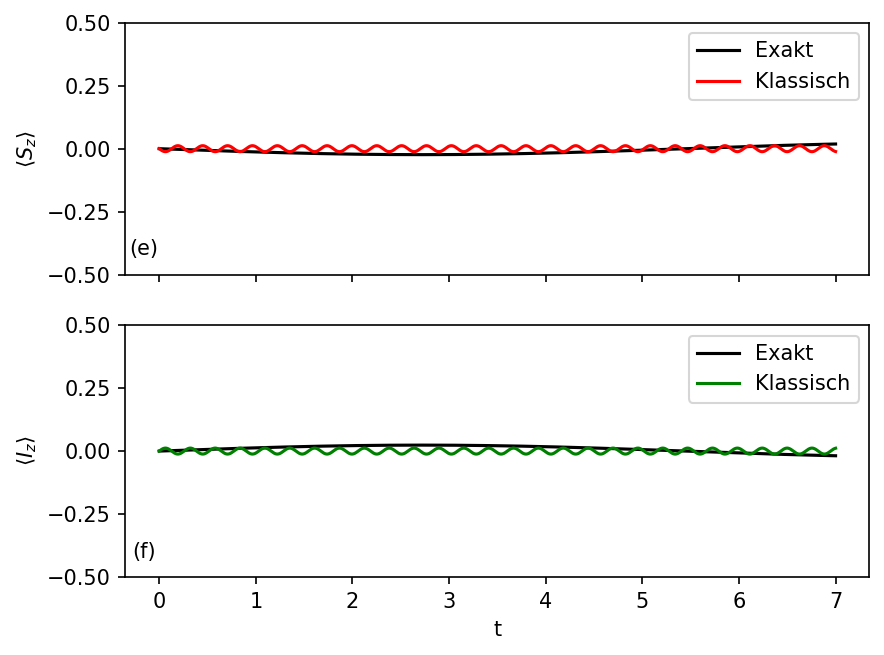
\includegraphics[width = 0.45\textwidth]{Abbildungen/Plot_Sz_index.png}
    \caption{Spin-Erwartungswerte des Elektronenspins S (Rot) und des Kernspins (Grün) und der jeweils exakten quantenmechanischen Lösung
    (Schwarz) gegen die Zeit t aufgetragen für die Parameter: $B = 0.5$ T, $T^*= 1 \thinspace$ns, $A_k = \sqrt{\frac{4}{3}}\cdot 10^9 \frac{1}{s}$,
    $z=\frac{1}{800}$.}
    \label{fig:Plots_2D}
\end{figure}

Aus \autoref{fig:Plots_2D} Panel (e) und (f) ist sehr gut zu erkennen, dass durch die Heisenbergkopplung die Spinerwartungswerte $\langle\hat{S}_z \rangle$ 
und $\langle\hat{I}_z \rangle$ um den Nullpunkt oszillieren und sehr kleine Amplituden besitzen, worauf geschloßen werden kann, dass die 
Spins einigermaßen auf der X-Y-Ebene verweilen und die Frequenz der klassischen Lösung deutlich größer ist als bei der Exakten.
\begin{figure}[h!]
    \centering
    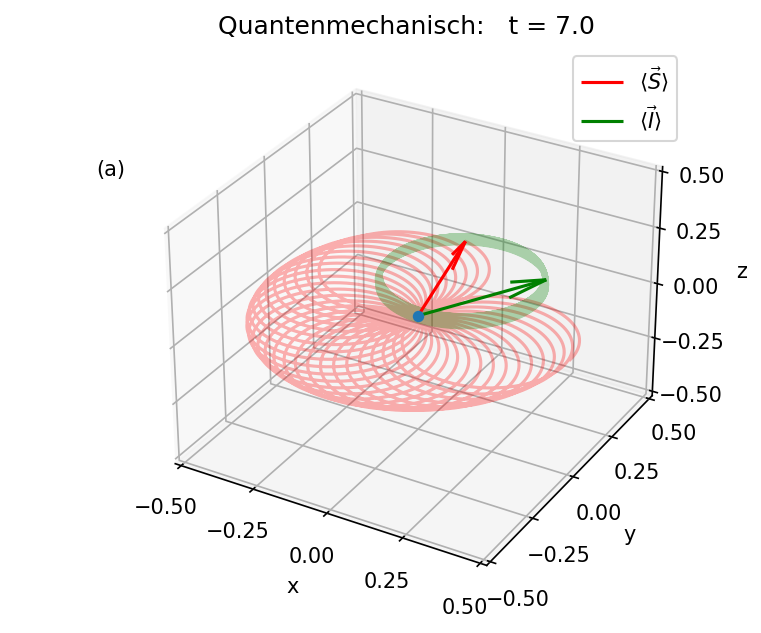
\includegraphics[width = 0.45\textwidth]{Abbildungen/Plot_Vektor_Quant_index.png}
    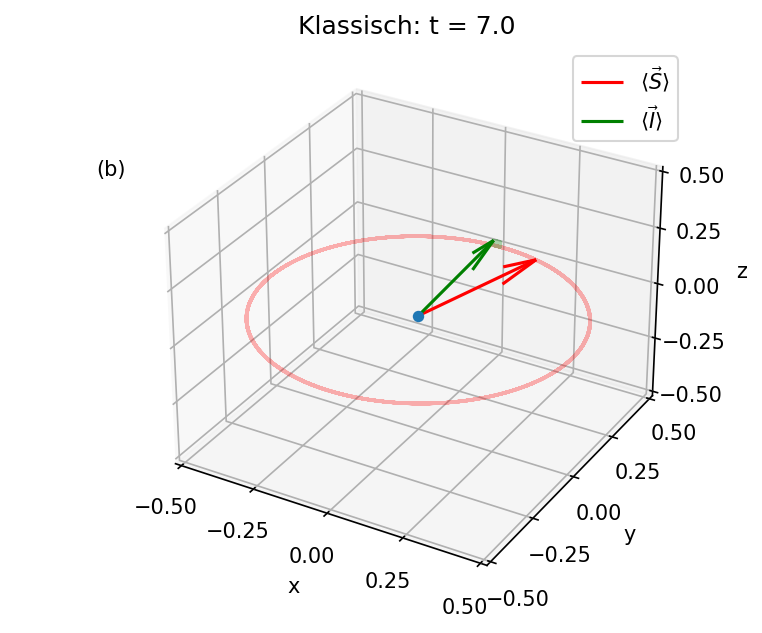
\includegraphics[width = 0.45\textwidth]{Abbildungen/Plot_Vektor_Klassisch_index.png}
    \caption{Spinerwartungswerte als Vektoren zum Endzeitpunkt des betrachten Zeitraums zum genannten Startzustand samt abgefahrener Spur der
    quantenmechanischen Lösung (Links) und der klassischen Lösung (Rechts) für die Parameter: $B = 0.5$ T, $T^*= 1 \thinspace$ns, $A_k = \sqrt{\frac{4}{3}}\cdot 10^9 \frac{1}{s}$,
    $z=\frac{1}{800}$.}
    \label{fig:Plots_3D}
\end{figure}
% Kreisbahnen als Verschränkung. Kreiszentren präzedieren. Kreiszentrumposition aus logischen gründen anhand der addierten Spinlänge erkennbar.

Wie für die klassische Lösung zu erwarten, präzedieren Elektronen- und Kernspin um das in z-Achse ausgerichtete Magnetfeld, wobei durch die stärkere Kopplung
die Larmorfrequenz für das Elektron deutlich größer ist. Dies macht sich besonders deutlich in \autoref{fig:Plots_2D} Panel (b) und (d), wo die grüne 
Kurve (Kernspin) einer Geraden gleicht und zeitglich in Panel (a) und (c) im selben Zeitintervall die rote Kurve (Elektron) mehrere Oszilattionen vollführt; 
oder wie in \autoref{fig:Plots_3D} Panel (b), wo der grüne Spurverlauf (Kernspin) marginal kurz ist im Vergleich zur roten Kreisspur (Elektron), 
in der der Elektronenspin schon mindestens eine Kreisbahn abgefahren ist.\\ 
\begin{figure}[h]
    \centering
    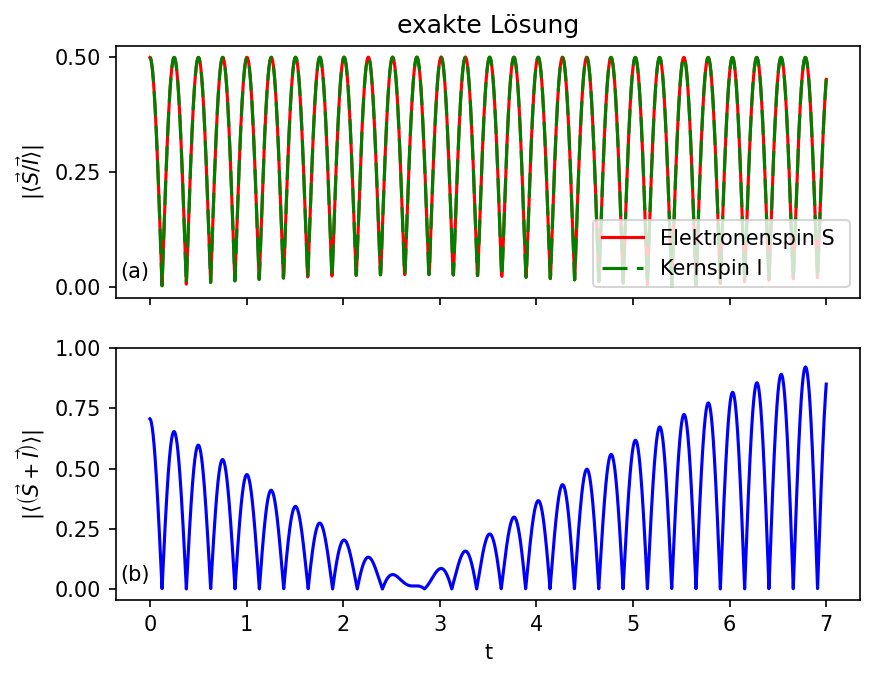
\includegraphics[width = 0.45\textwidth]{Abbildungen/Plot_Spin_length_index.png}
    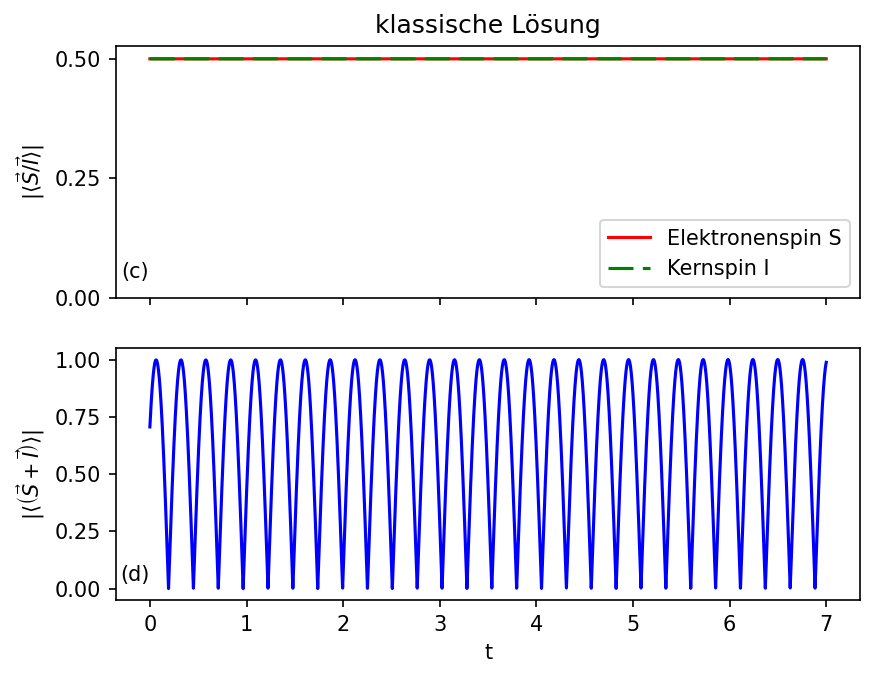
\includegraphics[width = 0.45\textwidth]{Abbildungen/Plot_Spin_length_Klassisch_index.png}
    \caption{Spinlängen-Erwartungswert der Einzelspins und addierten Spins des Kern-und Elektronenspins der exakten Lösung(links) und der klassischen 
    Lösung(rechts) gegen die Zeit aufgetragen für die Parameter: $B = 0.5$ T, $T^*= 1 \thinspace$ns, $A_k = \sqrt{\frac{4}{3}}\cdot 10^9 \frac{1}{s}$,
    $z=\frac{1}{800}$.}
    \label{fig:Plots_Spinlength}
\end{figure}
\noindent Die exakte Lösung berücksichtigt die Verschränkung beider Spins, welches sich hauptaugenscheinlich durch Veränderungen der Einzelspinlängen ausdrückt 
wie in \autoref{fig:Plots_Spinlength} Panel (a) und (b) zu sehen. Dabei sind beide Spinlängen in den Panels (a)  zu jedem Zeitpunkt identisch, was am totalen 
Überlappen beider Plots zu sehen ist; dasselbe gilt auch für den klassischen Fall in Panel (c), wobei die Spinlängen konstant bei 0.5 bleiben.\\
In \autoref{fig:Plots_3D} ist sehr gut zu erkennen, dass anders als im klassischen Fall (Panel (b)) die Spins im quantenmechanischem Fall (Panel (a)) 
Kreisbahnen abfahren, dessen Mittelpunkte nicht im Ursprung liegen, sondern gerade mittig zwischen Ursprung und maximaler Spinlänge. Trotzdessen ist eine Larmor-Präzessionsbewegung wie im Klassischen 
zu beobachten, in der nicht die Spinerwartungswerte präzedieren, sondern die jeweiligen Kreismittelpunkte, was zu den charakteristschen Schlaufen führt.\\
Dabei präzediert der Elektronenspin wie zu erwarten um einiges schneller als der schwachgekoppelte Kernspin um das Magnetfeld, welches gut in der 
ausgeprägten Schlaufenbildung in \autoref{fig:Plots_3D} Panel (a) zu sehen ist. 

Über \autoref{fig:Plots_3D} Panel (a) lässt sich anschaulich erklären, wie sich der zeitliche Verlauf der 
Spinlängen $|\langle \left( \vec{S}+\vec{I} \right)\rangle |$ der exakten Lösung in \autoref{fig:Plots_Spinlength} in Panel (b) zu Stande kommt. Die 
addierten Spinlängen oszillieren und sind von einer Umhüllenden umschlossen, die ihr Minimum bei etwa $t=3$ besitzt. Dies entspricht in etwa der halben Zeitdauer
des betrachteten Intervalls, woraus sich abschätzen lässt, dass in \autoref{fig:Plots_3D} Panel (a) der Elektronenspin den halben Schlaufenverlauf erst 
abgefahren ist. \\
Dort liegen die Kreiszentren des Elektronenspin- und Kernspinerwartungswert gegenüber, wodurch sie nur antiparallele
und keine parallelen Komponeneten teilen und sich in der Vektorsumme kürzen. Eine analoge Betrachtung erklärt, deshalb warum die addierte Spinlänge
jeweils an den beiden Enden des Zeitintervall über die Einzel-Spinlänge von 0.5 wächst.\\
In \autoref{fig:Plots_Spinlength} Panel (c) wird nochmal verdeutlicht, dass die Einzeilspinlängen in der klassischen Lösung konstant bleiben, aber es in 
Panel (d) bei der addierten Spinlänge zu Oszillationen kommt, die von der Larmor-Frequenzdifferenz abhängen. 

\chapter{Zusammenfassung}
% Was wurde erreicht
Zusammenfassend konnte nachegewiesen werden, dass das TDVP mit dem klassischen Ansatz Gl. (\ref{klassischer_Ansatz}) die klassischen Lösungen reproduzieren 
konnte, in der die Spinlängen konstant bleiben. Dadurch ist zu erkennen, dass der vom klassischen Ansatz beschränkte Unterraum des Hilbertraumes zu klein
ist, um die exakte Dynamik wiedergeben zu können. Die Erweiterung auf $n$ 1/2-Spins folgt durch den Produktansatz immer in analogen Schritten.\\
Wird bei den Ergebnissen des modifizierten Ansatzes der Korrekturparameter $\mu_{12}=0$ gesetzt, zerfallen wie zu erwarten
die Gram-Matrix Gl. (\ref{Gram_Korrektur}) und die partiellen Ableitungen der effektiven Hamilton-Funktion Gl. (\ref{dH_Q1}) bis Gl. (\ref{dH_Q12})
in die klassischen Lösungen.\\

Im Rahmen dieser Bachelorarbeit wurde die Lösung der Differentialgleichungen Gl. (\ref{QK_DGL1}) bis Gl. (\ref{QK_DGL3}) nicht behandelt. Es ist 
aber naheliegend, da der modifizierte Ansatz den ganzen Hilbertraum abdeckt, sich die exakte Lösung reproduzieren lässt. Dadurch würde sich 
mit Ausblick zukünftiger Arbeiten, die sich mit diesem Thema beschäftigen, die Überprüfung der Exaktheit dieser Lösung als zentrale Aufgabenstellung ergeben. \\
Für den Fall, dass die Exaktheit erfolgreich nachgewiesen wurde, wäre die Erweiterung auf 1/2-Spin-Systeme mit auf $n$ Spins die zentrale Aufgabe, 
denn dann dürften diese Korrekturparameter nicht mehr den gesamte Hilbertraum abdecken und Fehler sind höchstwahrscheinlich unvermeidbar. 
Da aber das zentrale Ziel den Rechenaufwand eines zu $n$ exponentiell anwachsenden Hilbertraumes zu umgehen ist, ist 
ein gewisser Fehler tolerierbar und eventuell durch eine besondere Wahl von Quantenkorrekturparameter minimierbar. Anknüpfend würde ein Vergleich mit 
anderen semiklassischen Ansätzen sinnvoll sein.


\appendix
% Hier beginnt der Anhang, nummeriert in lateinischen Buchstaben
%\input{content/a_anhang.tex}

\backmatter
\printbibliography

\cleardoublepage
% From https://www.tu-dortmund.de/studierende/im-studium/pruefungsangelegenheiten/allgemeine-vordrucke/
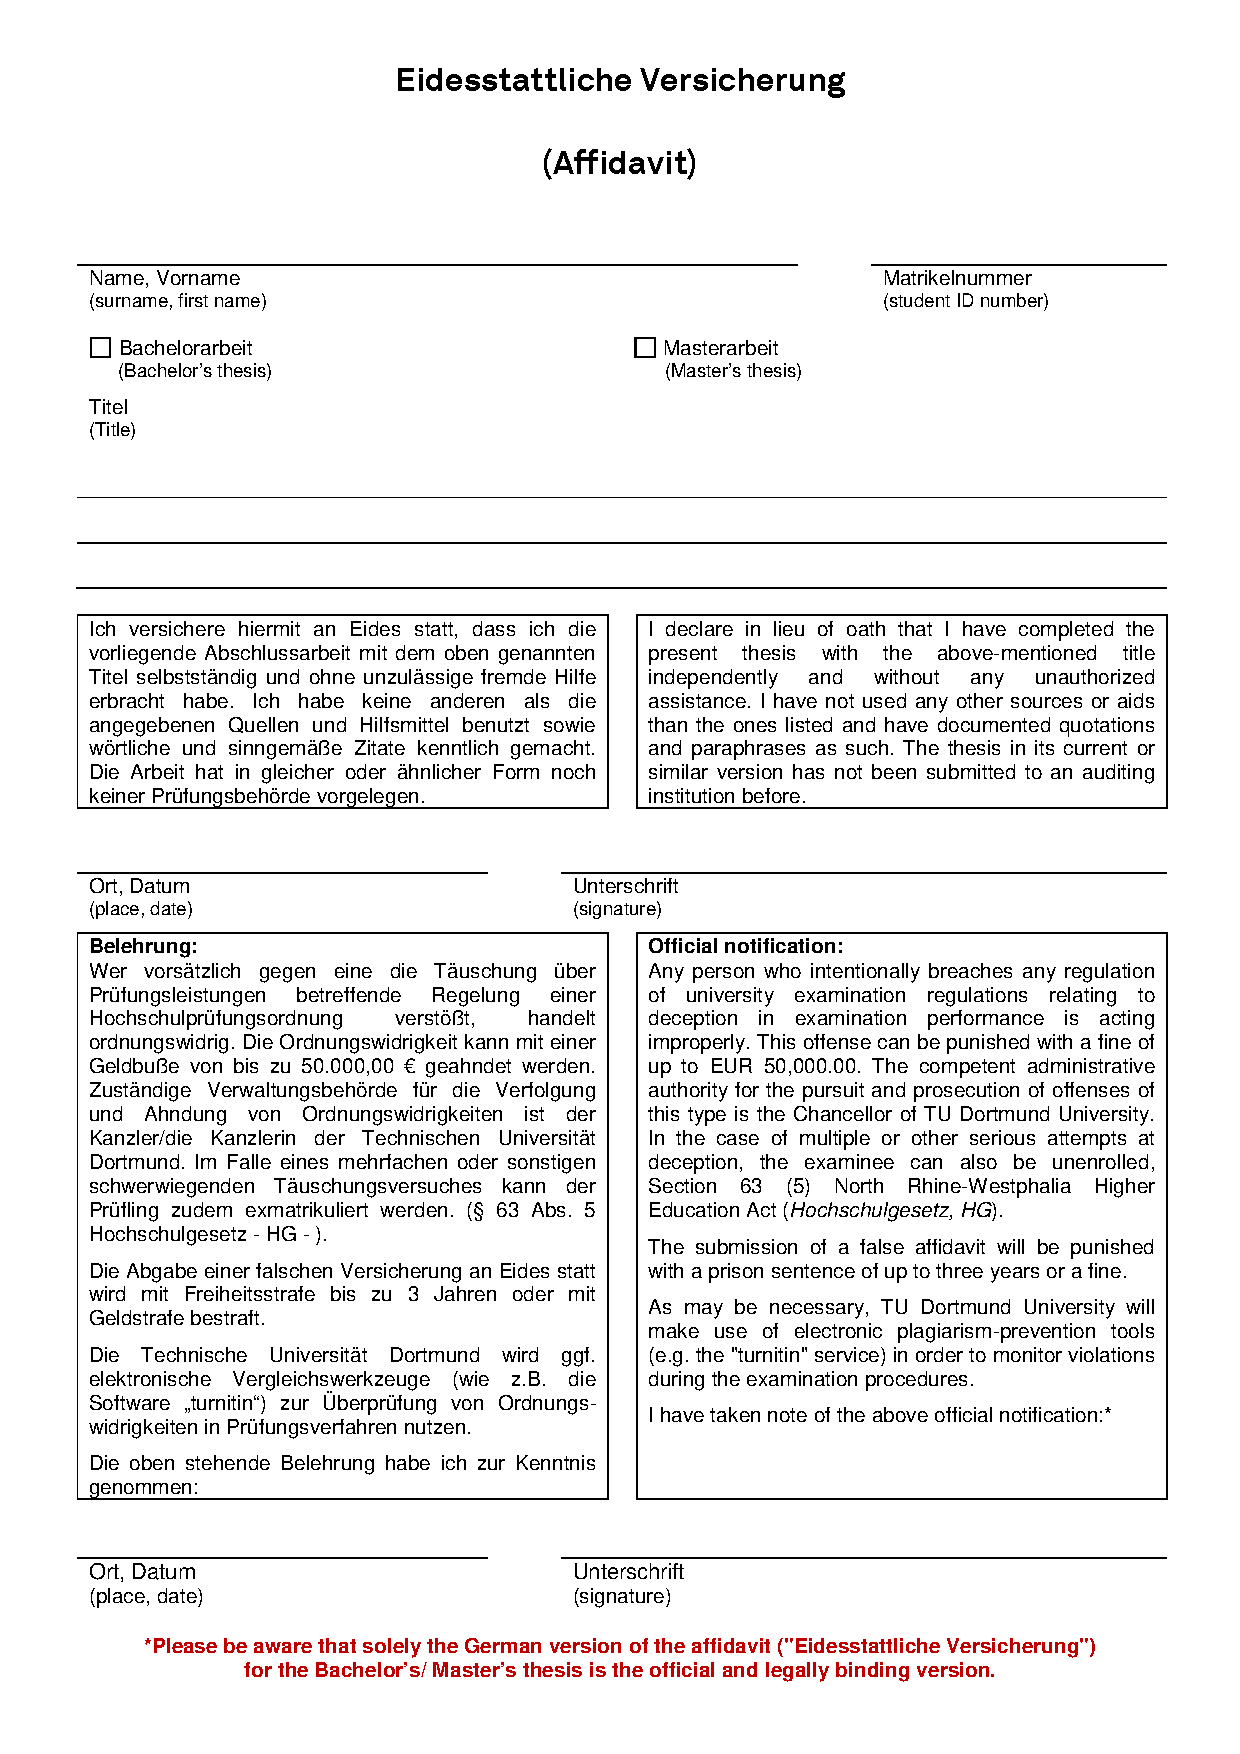
\includepdf{content/Eidesstattliche_Versicherung.pdf}

\end{document}


Dafür wird zuerst 
\begin{align}
    \partial_\mu \left(\frac{\bra{\Psi}\hat{S_x}\ket{\Psi}}{\N}\right)\dot{\mu} &= \frac{1}{2}\frac{1-\muk^2}{(1+\mu\muk)^2}\cdot\left[\frac{1}{2}(b_y + ib_x)\mu^2 + \frac{1}{2}(b_y - ib_x) +i\mu b_z\right] 
\end{align}
berechnet, um es dann in die Identität \ref{dS_dt} einzusetzen:
\begin{align}
    \frac{d}{dt}\left(\frac{\bra{\Psi}\hat{S_x}\ket{\Psi}}{\N}\right) &= \partial_{\mu}\left[\frac{\bra{\Psi}\hat{S_x}\ket{\Psi}}{\N}\right]\dot{\mu} + \partial_{\muk}\left[\frac{\bra{\Psi}\hat{S_x}\ket{\Psi}}{\N}\right]\dot{\muk}\\
    &= b_y \frac{1}{2}\frac{1-\mu\muk}{(1+\mu\muk)^2} - b_z \frac{i}{2}\frac{\muk -\mu}{(1+\mu\muk)^2}    \\
    &= b_y\left(\frac{\bra{\Psi}\hat{S_z}\ket{\Psi}}{\N}\right) - b_z\left(\frac{\bra{\Psi}\hat{S_z}\ket{\Psi}}{\N}\right)
\end{align}
analog wird berechnet:
\begin{align}
    \frac{d}{dt}\left(\frac{\bra{\Psi}\hat{S_y}\ket{\Psi}}{\N}\right) &= b_z\left(\frac{\bra{\Psi}\hat{S_x}\ket{\Psi}}{\N}\right) - b_x\left(\frac{\bra{\Psi}\hat{S_z}\ket{\Psi}}{\N}\right)\\
    \frac{d}{dt}\left(\frac{\bra{\Psi}\hat{S_z}\ket{\Psi}}{\N}\right) &= b_x\left(\frac{\bra{\Psi}\hat{S_y}\ket{\Psi}}{\N}\right) - b_y\left(\frac{\bra{\Psi}\hat{S_x}\ket{\Psi}}{\N}\right)
\end{align}
Die Kreuzproduktstruktur lässt sich somit wiedererkennen.

